%%%%% Please set the path to 'beamer' directory in your environment %%%%%
\newcommand{\beamerDir}[0]{/mnt/c/Users/atsushi/Documents/workspace/env/Beamer/beamer/beamer/}


%%%%% Load setting %%%%%
\documentclass[aspectratio=169, dvipdfmx, 12pt, compress]{beamer}% dvipdfmxしたい

%%%%% Packages %%%%%
\usepackage{bxdpx-beamer}% dvipdfmxなので必要
\usepackage{pxjahyper}% 日本語で'しおり'したい
\usepackage{tikz}
\usepackage{tcolorbox}
\usetikzlibrary{shapes}
\usepackage{xcolor}
\usepackage[absolute,overlay]{textpos}
\usepackage{adjustbox}
\usepackage{caption}
\usepackage{ifthen}


%%%%% Settings %%%%%
\usetheme[sectionpage=progressbar, subsectionpage=progressbar]{metropolis}
% block style
\metroset{block=fill}
% space between line
\renewcommand{\baselinestretch}{1.3}
% space between item
\newlength{\wideitemsep}
\setlength{\wideitemsep}{0.9\itemsep}
% \addtolength{\wideitemsep}{1.0pt} <- more space
\let\olditem\item
\renewcommand{\item}{\setlength{\itemsep}{\wideitemsep}\olditem}
% frame title
\definecolor{coolblack}{rgb}{0.0, 0.18, 0.39}
\setbeamercolor{frametitle}{bg=coolblack!90,fg=white}
\setbeamerfont{frametitle}{size=\large}
\addtobeamertemplate{frametitle}{}{\vspace{-1em}}
\makeatletter
\setlength{\metropolis@frametitle@padding}{1.4ex}% <- default 2.2 ex
% foot line
\addtobeamertemplate{footline}{}{\vspace{-1em}}
% normal text color
\setbeamercolor{normal text}{fg=black!80}
% progress bar
\definecolor{lightgray}{rgb}{0.83, 0.83, 0.83}
\setbeamercolor{progress bar}{bg=lightgray, fg=coolblack}
\setbeamersize{text margin left=15pt, text margin right=15pt}
% equation font
\usefonttheme{professionalfonts}
% Change standard block width
\addtobeamertemplate{block begin}{%
    \centering
    \begin{columns}\begin{column}{0.9\textwidth}
            \centering
            }{}
            \addtobeamertemplate{block end}{}{\end{column}\end{columns}}
% Change alert block width
\addtobeamertemplate{block alerted begin}{%
    \centering
    \begin{columns}\begin{column}{0.9\textwidth}
            \centering
            }{}
            \addtobeamertemplate{block alerted end}{}{\end{column}\end{columns}}
% Change example block width
\addtobeamertemplate{block example begin}{%
    \centering
    \begin{columns}\begin{column}{0.9\textwidth}
            \centering
            }{}
            \addtobeamertemplate{block example end}{}{\end{column}\end{columns}}
% Itemize color
\setbeamertemplate{itemize item}{\color{black}\scriptsize$\blacksquare$}
\setbeamertemplate{itemize subitem}{\color{black}\scriptsize$-$}
% Simplification  color
\definecolor{cobalt}{rgb}{0.0, 0.28, 0.67}
\setbeamercolor{block title example}{fg=black!80,bg=cobalt!35}
\setbeamercolor{block body example}{fg=black,bg=cobalt!15}
% Definition
\BeforeBeginEnvironment{definition}{
    \setbeamercolor{block title}{use=alerted text, bg=alerted text.fg!70,fg=white}
    \setbeamercolor{block body}{use=alerted text, bg=alerted text.fg!20}
}
\AfterEndEnvironment{definition}{% return to default
    \setbeamercolor{block title}{use=structure,fg=structure.fg,bg=structure.fg!20!bg}
    \setbeamercolor{block body}{parent=normal text,use=block title,bg=block title.bg!50!bg, fg=black}
}
% Theorem
\definecolor{seagreen}{rgb}{0.18, 0.55, 0.34}
\setbeamertemplate{theorems}[numbered]
\BeforeBeginEnvironment{theorem}{
    \setbeamercolor{block title}{fg=black!80,bg=seagreen!40}
    \setbeamercolor{block body}{fg=black,bg=seagreen!15}
}
\AfterEndEnvironment{theorem}{% return to default
    \setbeamercolor{block title}{use=structure,fg=structure.fg,bg=structure.fg!20!bg}
    \setbeamercolor{block body}{parent=normal text,use=block title,bg=block title.bg!50!bg, fg=black}
}
% Lemma
\undef{\lemma}
\newtheorem{lemma}{\translate{Lemma}}
\BeforeBeginEnvironment{lemma}{
    \setbeamercolor{block title}{fg=black!80,bg=seagreen!20}
    \setbeamercolor{block body}{fg=black,bg=seagreen!10}
}
\AfterEndEnvironment{lemma}{% return to default
    \setbeamercolor{block title}{use=structure,fg=structure.fg!80,bg=structure.fg!20!bg}
    \setbeamercolor{block body}{parent=normal text,use=block title,bg=block title.bg!50!bg, fg=black}
}


%%%%% Original Command %%%%%
\newcommand{\subt}[1]{\vspace{-2mm}{\fontsize{10pt}{0cm}\selectfont \textcolor{lightgray}{#1}}\vspace{-1mm}}
\newcommand{\lastpage}[0]{\begin{frame}\begin{textblock*}{1.0\linewidth}(0pt, 50pt)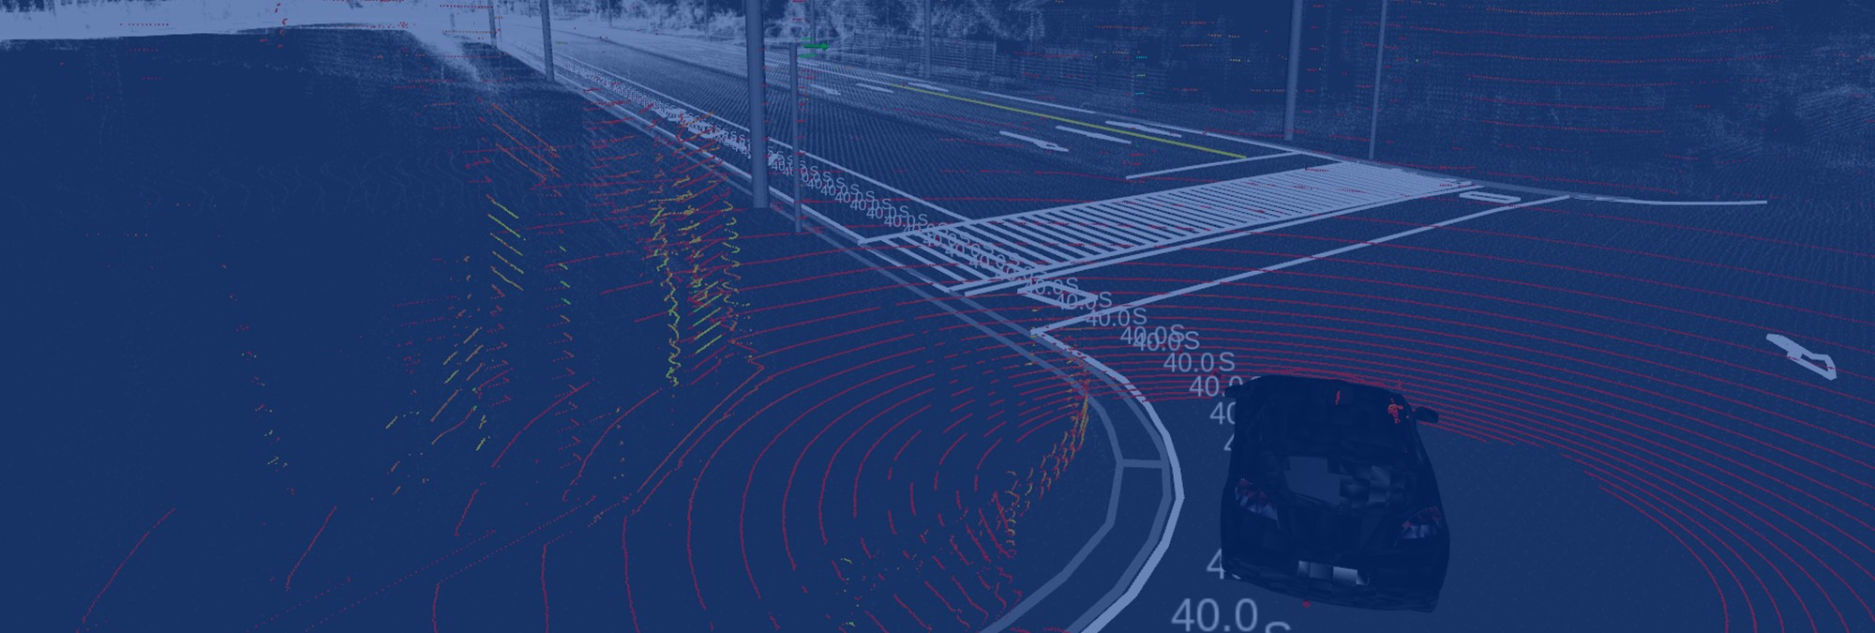
\includegraphics[scale=0.512]{\beamerDir/master_figure/last.pdf}\end{textblock*}\end{frame}}
\newcommand{\todo}[1]{\al{\LARGE\textbf{TODO:} #1}}
\newcommand{\headerheight}[0]{5mm}
\newcommand{\footerheight}[0]{5mm}
\newcommand{\slideheight}[0]{\textheight-\headerheight-\footerheight}
\newcommand{\tabml}[1]{\hspace{-2.1mm}\begin{tabular}{l} #1 \end{tabular}}
\newcommand{\al}[1]{\alert{#1}}
\newcommand{\argempty}[0]{}
\newcommand{\onlyslide}[1]{
    \vspace{\headerheight}
    \begin{minipage}[c][\slideheight][c]{\textwidth}
        #1
    \end{minipage}
}
\newcommand{\onlyimage}[1]{
    \onlyslide{
        \centering
        \begin{columns}
            \begin{column}{\textwidth}
                \centering
                \adjustbox{max width=\textwidth, max height=\slideheight}{
                    \includegraphics{#1}
                }
            \end{column}
        \end{columns}
    }
}
% fit image
\newlength\fitimageht
\newlength\fitotherht
\newsavebox\fitimagebox
\newcommand{\fitimage}[2]{%
    \sbox\fitimagebox{%
        \parbox{\textwidth}{%
            #1\par
        }%
    }%
    \settototalheight{\fitotherht}{%
        \usebox\fitimagebox
    }%
    \setlength\fitimageht{\textheight}%
    \addtolength\fitimageht{-\fitotherht-\headerheight-\footerheight-1\baselineskip}%
    \vspace{\headerheight}
    #1\par
    \centering
    \includegraphics[width=\textwidth,height=\fitimageht,keepaspectratio]{#2}
}
% Simplification
\newcommand{\assume}[1]{
    \begin{exampleblock}{Simplification }
        #1
    \end{exampleblock}
}
% Re-post
\setbeamercolor{RepostBox}{fg=black!50, bg=coolblack!10}
\newcommand{\repost}[1]{
    \vspace{2mm}
    \centering
    \begin{columns}
        \begin{column}{0.86\textwidth}
            \begin{beamercolorbox}[wd=\textwidth, sep=2pt, rounded=true, shadow=true]{RepostBox}
                \begin{tabular}{|p{0.95\textwidth}}
                    {\fontsize{10pt}{10pt}#1}
                \end{tabular}
            \end{beamercolorbox}
        \end{column}
    \end{columns}
}

% equation ballon
\tcbset{
    framebox/.style={
            enhanced,
            boxsep=0pt,       % 箱の上下左右の余白を指定
            colback=white,
            boxrule=1pt,
            colframe=#1
        },
    framebox/.default=red
}
\newcommand{\upbln}[3]{
    \tcboxmath[
        framebox=#2,
        top=0.5ex,bottom=0.5ex,    % 箱の上下の余白を指定
        left=0.5ex,right=0.5ex,    % 箱の左右の余白を指定
        overlay={
                \node[
                    above,
                    rectangle callout,                         % nodeを吹き出しの形に
                    callout absolute pointer={(frame.north)},  % 吹き出しの先端を絶対的に指定
                    fill=#2!20
                ] at ([yshift=2ex]frame.north) {\footnotesize#3};
            }
    ]{#1}
}
\newcommand{\lwbln}[3]{
    \tcboxmath[
        framebox=#2,
        top=0.5ex,bottom=0.5ex,    % 箱の上下の余白を指定
        left=0.5ex,right=0.5ex,    % 箱の左右の余白を指定
        overlay={
                \node[
                    below,
                    rectangle callout,                         % nodeを吹き出しの形に
                    callout absolute pointer={(frame.south)},  % 吹き出しの先端を絶対的に指定
                    fill=#2!20
                ] at ([yshift=-2ex]frame.south) {\footnotesize#3};
            }
    ]{#1}
}
\tcbuselibrary{theorems,skins}



%%%%% Front Cover %%%%%
\title{Real-Time Scheduling and Analysis of Processing Chains on Multi-threaded Executor in ROS 2}
\subtitle{2022 RTSS}
\author{矢野 篤志}
\date{\today}
\institute[EMBIV]{EMBIV}
\logo{\begin{textblock*}{0.1\linewidth}(2pt, 237pt)
\includegraphics[scale=0.4]{\beamerDir/master_figure/Emb_logo.pdf}\end{textblock*}}


%%%%% Document Start %%%%%
\begin{document}

\maketitle

% !TeX root = main.tex


\begin{frame}{提案の概要}
    \begin{itemize}
        \item 優先度駆動型スケジューリングによってROSのリアルタイム性能と予測可能性を大幅に改善できることを主張する
        \item 主張を裏付けるために, 優先度駆動型チェーン考慮スケジューリングに関する我々の研究をレビューし, Apex.AI が開発したオープンソースリファレンスシステムを用いた評価を行う
        \item ROS 2のリアルタイム性能を向上させるために不可欠な以下2つの課題を説明する
        \begin{itemize}
            \item マルチスレッドエグゼキュータ設計
            \item アクセラレータサポート
        \end{itemize}
    \end{itemize}
\end{frame}


\begin{frame}{Outline}
    \setbeamertemplate{section in toc}[sections numbered]
    \scriptsize\tableofcontents[hideallsubsections]
\end{frame}

% !TeX root = main.tex

\section{INTRODUCTION}
\label{sec: introduction}

\begin{frame}{}
    \begin{itemize}
        \item ロボット工学のような, 様々な分野の深い専門知識を必要とする学際的で複雑なアプリケーション領域では, 通常, 全ての, あるいはほとんどのソフトウェアをゼロから書くという選択肢はあり得ない
        \item その代わりに, ロボット工学者は, ROSのような一般的なロボット工学フレームワークで容易に利用できる, 標準機能を提供する既存のサードパーティコンポーネントの統合を採用するのが一般的である
        \item その利点は数多く, 簡単に理解できる
        \item 例えば, 複数の最新パス計画アルゴリズムと3D可視化サポートを備えた完全なナビゲーションスタックがたった1回のダウンロードで手に入るなら, なぜ新しいナビゲーションサブシステムを苦労して開発する必要があるか?
    \end{itemize}
\end{frame}

\begin{frame}{}
    \begin{itemize}
        \item 完全なロボットシステムを構築するためには, 多くの相互作用するコンポーネントを統合する必要がある
        \item ROS開発プロセスの分散型オープンソースの性質により, これらのコンポーネントは通常, 必ずしもお互いを知らない複数の独立したコンポーネント開発者によって分離して開発される
        \item 同様に, システムインテグレータは, アプリケーションおよびミッション固有のロジックと「グルーコード」で展開プラットフォーム上で選択したコンポーネントを構成するが, 通常, それぞれのコンポーネント開発者と密接に連携することはない
    \end{itemize}
\end{frame}

\begin{frame}{}
    \begin{itemize}
        \item コンポーネントの統合を可能な限りシンプルに保つために, ROSはコンポーネントの疎結合を可能にする古典的なトピックベースのpublish/subscribeパラダイムを採用している
        \item 概念的には, 各コンポーネントは, 特定のトピックをsubscribeする多数のコールバックを含む「ブラックボックス」として理解できる
        \item 与えられたトピックに関連するメッセージがpublishされるたびに, 全てのsubscribeコールバックが呼び出され, 何らかの計算を実行し, 次に他のトピックに後続のメッセージをpublishすることができ, これがさらにコールバックをトリガするというように, 繰り返す
    \end{itemize}
\end{frame}

\begin{frame}{}
    \begin{itemize}
        \item インテグレータは, あるコンポーネントの「入力コールバック」を別のコンポーネントの「出力トピック」に接続することによってコンポーネントを構成する
        \item ROSシステムは, このように相互接続されたトピックとコールバックの複雑なネットワークを形成し, データ (環境刺激など) は, イベント駆動型の方法でネットワークを通じてcause-effectチェーンに沿って伝播し, インテグレータが望むように透過的にコンポーネント境界を交差させることができる
    \end{itemize}
\end{frame}

\begin{frame}{}
    \begin{itemize}
        \item このようなcause-effectチェーンの典型的な例として, 進路上の障害物を検知して反応する必要のある移動ロボットのセンシング-計算-行動パイプラインが挙げられる
        \item 例えば, ハードウェアドライバコンポーネントがレーザースキャナから新しいサンプルを取得し (cause) , それが複数のマッピング, 座標変換, パス計画, 車輪制御コンポーネントを経て, 最終的に車輪速度の変化 (effect) をもたらす可能性がある
        \item このようなデータ処理のチェーンにおいて, causeからeffectまでの最大レイテンシ時間は, ロボットが正しく機能するために重要な役割を果たすことは明らかであり, また, 安全性を考慮する上でも重要であることが多い
    \end{itemize}
\end{frame}

\begin{frame}{}
    \begin{itemize}
        \item 重要なのは, システムインテグレータにできるだけ多くの展開の選択肢を残し, コンポーネントの再利用の機会を最大化するために, ROSの実行管理層と基礎となるオペレーティングシステムは, 意図的にコンポーネント開発者に公開されないことである
        \item むしろ, ROSの中心的なコールバック抽象化は, コールバック手続きがいつどのようにスケジュールされるか, コールバックの実行がスレッドまたはプロセスにわたってどのように組織されるか, またはネットワーキング層がメッセージの送受信をどのように処理するかを全く意識せずに, 実行から完了までセマンティクスを持つ単なる手続きである
    \end{itemize}
\end{frame}

\begin{frame}{}
    \begin{itemize}
        \item ROSはオープンソースソフトウェアであるため, 原理的にはシステムの実行と通信の挙動を完全に理解し制御することが可能である
        \item このため, リアルタイムシステムの専門家から見れば, ROSにリアルタイムシステム研究でよく知られた技術を導入することは論理的なステップであるように思える可能性がある
        \item しかし, 一見したところ, これを難しくしているハードルがいくつかある
    \end{itemize}
\end{frame}

\begin{frame}{}
    \begin{itemize}
        \item まず第一に, インテグレータに必要な情報が不足している
        \item ほとんどのリアルタイム分析では, 同時実行タスクの数, それらの起動セマンティクスや機能的相互作用, メッセージの到着パターン, 最悪実行時間など, 多くの低レベルシステムの詳細に関する深い知識が前提となっている
        \item ROSコンポーネントは, この種の情報を提供するマニフェストと一緒に来ることはない
        \item さらに悪いことに, リアルタイム分析は, 欠陥のある情報や不完全な情報にうまく対処できない
        \item モデリング目的でサードパーティコンポーネントを手作業でリバースエンジニアリングしているときに, たった一つのミスや見落としがあれば, その取り組み全体を無条件に無効にしてしまうことになりかねない
    \end{itemize}
\end{frame}

\begin{frame}{}
    \begin{itemize}
        \item 第二に, 必要なシステムの詳細をコンポーネントレベルで静的に決定し, 記述することができない
        \item その理由のひとつは, 多くのロボット工学アルゴリズムが, ユースケースやプラットフォーム固有の側面に依存し, 実行時間や起動パターンが大きく変化するためである
        \item 例えば, ビデオストリーム中の物体を識別し, その軌跡を推測する一般的な物体追跡コンポーネントを考えてみよう (例えば, 隣の車線の車など)
        \item この機能の実行時間は, ビデオストリームのフレームレート, 解像度, コーデック, および特定のトラッキングアルゴリズムに関連する他の様々なパラメータを含む, 様々なパラメータに依存する
        \item これらのパラメータは, 一般的なオブジェクトトラッキングコンポーネントの開発者が前もって知っていたり, 固定されていたりするものではない
    \end{itemize}
\end{frame}

\begin{frame}{}
    \begin{itemize}
        \item このようなユースケース特有の情報は, 特定のロボットを構築するインテグレーターにしか分からない
        \item インテグレーターは, 必ずしもオブジェクトトラッキングやリアルタイムシステムの専門家ではないため, 特定の構成を選択した場合の影響を常に予測できるわけではない
        \item したがって, コンポーネントのリソース要求とリアルタイム動作は, 常に特定の展開で使用するという文脈で評価されなければならない
        \item これは, ROSフレームワークの人気の根底にある「ブラックボックス」コンポーネントのモジュール式再利用と相容れるものではない
    \end{itemize}
\end{frame}

\begin{frame}{}
    \begin{itemize}
        \item 最後に, 仮にインテグレータが各コンポーネントについてそれぞれの専門家と議論し, タイミング分析に必要な全ての詳細を入手できたとしても, 第三の根本的な問題が残る
        \item 多くのコンポーネントのリソース要件と性能特性は, 本質的にロボットの動的環境に依存し, したがって時間とともに変化するため, 静的 (最悪のケース) リソース配置は実行不可能なのである
    \end{itemize}
\end{frame}

\begin{frame}{}
    \begin{itemize}
        \item 例えば, 前述の物体追跡コンポーネントと, ランドマークベースの自己位置特定コンポーネントに依存するロボットを再度考えてみよう
        \item 一方, 人口が少ない田舎町よりも, にぎやかな街中を移動する方が, 物体追跡装置の処理時間はずっと長くなる
        \item 一方, 認識可能なランドマークが多い都市部では, ほぼ一様な風景よりも自己位置推定がはるかに容易である可能性が高い
        \item どちらの状況でも十分なリソースを確保するためには, システムインテグレーターは, 不毛の土地からなる賑やかな都市を想定したシステムを用意しなければならない
    \end{itemize}
\end{frame}

\begin{frame}{}
    \begin{itemize}
        \item ロボット工学では, このような悲観的なシステム設計を行うと, すぐに現実的な限界に直面することになる
        \item その代わりに, 実用的で費用対効果の高いシステムを維持するためには, 各コンポーネントのピーク需要の合計ではなく, 予想されるジョイントリソースのピーク需要に対してプロビジョニングを行う必要がある
    \end{itemize}
\end{frame}

\begin{frame}{貢献する}
    \begin{itemize}
        \item これらの課題を克服するために, 我々は, 実行時に動的にタイミングを考慮した方法でROSシステムをプロビジョニングするための自動レイテンシマネージャを使用することを提案する
        \item 具体的には, ROS Live latency manager (ROSLlama) を紹介する
        \item これは, 重要なcause-effectチェーンに沿ったレイテンシを, 非リアルタイム専門家が使いやすく, かつ設定にあまり手間をかけない方法で, 既存のリアルタイム機構を使用して制御することを可能にする
    \end{itemize}
\end{frame}

\begin{frame}{貢献する}
    \begin{itemize}
        \item ROS-Llamaは, 複雑なシステムパラメータをユーザに要求するのではなく, 実行時に必要なパラメータを自動的に推定し, 状況の変化に応じてスケジューリングパラメータを動的に調整することが可能である
        \item もし, 指定されたレイテンシの目標が全て同時に達成できない場合 (例えば, 不利な環境条件による一時的な過負荷が原因) , ROS-Llamaは制御された緩やかなデグレードプロセスを開始し, システムインテグレーターが純粋に宣言的な方法で (すなわち, cause-effectチェーンがどの部品を通過しているかを理解しなくても) cause-effectチェーンの重要性を特定できるようにする
    \end{itemize}
\end{frame}

\begin{frame}{本論文の貢献}
    \begin{itemize}
        \item  ロボティクス領域における動的レイテンシ管理問題を探求し, 実用的なソリューションが満たさなければならない制約と要件を文書化する (第III章)

        \item  ROSのための最初の自動レイテンシマネージャであるROS-Llamaの設計と実装を紹介する (セクションIV)

        \item 標準的な Linux システム上の ROS コンポーネントを用いて, ROS-Llama が移動ロボットのcause-effectチェーンのレイテンシをうまく制御できることを示す評価について報告する (セクションVI)

    \end{itemize}
\end{frame}

\begin{frame}{}
    \begin{itemize}
        \item ROS-Llamaは, 数年にわたる研究とエンジニアリングの努力の結果であり, その間, 我々は多くの課題や技術的な限界に遭遇した
        \item セクションVIIでは, 以下の点を強調する
              \begin{itemize}
                  \item  ROS-Llamaをより効果的かつ正確にするための分析改善の機会
                  \item  ROSとLinuxのプラットフォームには, システムのさらなる改良の妨げとなる大きな限界がある
              \end{itemize}
    \end{itemize}
\end{frame}

% !TeX root = main.tex


\section{BACKGROUND}
\label{sec: background}


\subsection{ROS2}
\label{ssec: ros2}

\begin{frame}{ROS 2}
    \fitimage{
        \al{ROS 2} は OS 上の複数の抽象化レイヤの統合実装
    }{figure/ros2_system.png}
\end{frame}

\begin{frame}{Publish/Subscribeパラダイム}
    ROS 2 アプリケーションは, \al{publish/subscribeパラダイム}を使用して相互に通信する複数のノードで構成される

    \begin{block}{Publish/Subscribeパラダイム}
        \setlength{\linewidth}{0.98\columnwidth}
        \begin{itemize}
            \item ノードはトピックにメッセージをpublishし, そのトピックをsubscribeしているノードにメッセージをブロードキャストする
            \item ノードはコールバックをアクティブにして各メッセージを処理することにより, publish メッセージに反応する
            \item コールバックはメッセージ自体をpublishすることも可能で, 複雑な動作をトピックとコールバックのネットワークとして実装できる
        \end{itemize}
    \end{block}
\end{frame}

\begin{frame}{エグゼキュータ}
    \begin{itemize}
        \item ROS 2 アプリケーションがプラットフォームに展開される際には, 個々のノードが OS のプロセスにマップされる
        \item ROS 2 クライアントライブラリの\al{エグゼキュータ}は, OS プロセス内のノードのコールバックの実行を調整する
    \end{itemize}
\end{frame}

\begin{frame}{シングル/マルチスレッドエグゼキュータ}
    \begin{itemize}
        \item ROS 2 には以下 \tu{2 つの組み込みエグゼキュータがある}
              \begin{block}{シングルスレッドエグゼキュータ}
                  1 つのスレッドでコールバックを実行するエグゼキュータ
              \end{block}
              \begin{block}{マルチスレッドエグゼキュータ}
                  コールバックの処理を複数のスレッドに分散するエグゼキュータ
              \end{block}
              \vspace{5mm}

        \item \textbf{\underline{本論文ではマルチスレッドエグゼキュータに焦点を当てる}}
    \end{itemize}
\end{frame}

\begin{frame}{DDS (Data Distribution Service)}
    ノードのpublisherとsubscriberの間のメッセージ交換は, 抽象\al{DDS} (Data Distribution Service) 層によって実現される

    \begin{block}{抽象DDS}
        DDS とクライアントライブラリ間の通信インタフェース
    \end{block}
    \begin{block}{DDS}
        publisherとsubscriber間でメッセージを交換するための業界標準の分散通信システム
    \end{block}
\end{frame}

\begin{frame}{処理チェーン}
    \fitimage{
        \begin{itemize}
            \item \al{処理チェーン}は特定のイベントによってトリガされ, 複数のエグゼキュータにまたがる
            \item チェーンの各頂点はコールバックを表す
        \end{itemize}
    }{figure/multi_threaded_executor.png}
\end{frame}

\begin{frame}{本論文の分析の焦点}
    \fitimage{
        \tu{本論文では単一のエグゼキュータにおけるチェーンの応答時間に焦点を当てる}
        \notes{CPAアプローチ*によってチェーンが複数のエグゼキュータにまたがる場合に拡張できる}
    }{figure/multi_threaded_executor.png}

    \source{*D.Casini et al., “Response time analysis of ROS 2 processing chains under reservation-based scheduling,” in ECRTS, 2019.}
\end{frame}

\begin{frame}{コールバックグループ}
    \fitimage{
        \begin{itemize}
            \item コールバックは必ず1つの\al{コールバックグループ}に属す
            \item エグゼキュータ内のコールバックは, 異なるコールバックグループに属す可能性がある
        \end{itemize}
    }{figure/multi_threaded_executor.png}

\end{frame}

\begin{frame}{ノード}
    \begin{itemize}
        \item コールバックは異なる\al{ノード}に属す場合もある
        \item ROS 2 では, 同じノード内のコールバックはデフォルトで同じコールバックグループとなる
        \item これを除いて, ノードの概念は本論文とは無関係
    \end{itemize}

    \assume{簡単にするために, モデルにノードレベルの情報を含めない}
\end{frame}


\subsection{Scheduling of multi-threaded executor}
\label{ssec: scheduling_of_multi_threaded_executor}

\begin{frame}{}
    \begin{itemize}
        \item ROS 2 マルチスレッドエグゼキュータのスケジューリング動作を紹介する
        \item \tu{本論文の内容は ROS 2 Foxy Fitzroy に基づいている}
    \end{itemize}

\end{frame}

\begin{frame}{コールバック}
    \begin{itemize}
        \item \al{コールバック}は ROS 2 の最小のスケジューリングエンティティ
        \item マルチスレッドエグゼキュータでは, スレッドは抽象 DDS レイヤからメッセージを受け取り, 対応するコールバックを実行する
    \end{itemize}
\end{frame}

\begin{frame}{コールバックの優先順位決定方法}
    ROS 2 では, \tu{コールバックの優先度は 2 つのレベルで決定される}

    \begin{block}{コールバックタイプ}
        \setlength{\linewidth}{0.98\columnwidth}
        \begin{itemize}
            \item コールバックはタイマ・サブスクライバ・サービス・クライアントの 4 つのタイプに分類される
            \item 優先順位は, タイマ $\succ$ サブスクライバ $\succ$ サービス $\succ$ クライアント \notes{$\succ$: より高い優先度を持つ}
        \end{itemize}
    \end{block}

    \begin{block}{登録順}
        先に登録されたコールバックが優先される
    \end{block}
\end{frame}

\begin{frame}{コールバックタイプに関する簡単化}
    \full{
        \assume{本論文ではコールバックタイプに関する情報は含めない}
    }
\end{frame}

\begin{frame}{yield\_before\_execute}
    \begin{itemize}
        \item \al{yield\_before\_execute} が false に設定されている場合, スレッドは選択されたコールバックの実行をすぐに開始する
        \item yield\_before\_execute が true に設定されている場合, スレッドは再度スケジュールされるまでプロセッサを OS に譲る
        \item \tu{本論文ではデフォルトの設定である yield\_before\_execute $=$ false とする}
    \end{itemize}
\end{frame}

\begin{frame}{メッセージキュー}
    ROS 2 では, 各コールバックに到着したメッセージをバッファリングするためのキューがあり, その深さはユーザによって指定される
    \assume{
        \setlength{\linewidth}{0.98\columnwidth}
        \begin{itemize}
            \item キューが十分に大きく, メッセージが上書きされない
            \item コールバックは最も早く到着したメッセージでノンプリエンプティブに実行される
        \end{itemize}
    }
\end{frame}

\begin{frame}{wait\_set}
    エグゼキュータ内のスレッドは共通のセット \al{wait\_set} によって, 利用可能なメッセージを持つコールバックを保持する
\end{frame}

\begin{frame}{reentrant/mutually exclusiveコールバックグループ}
    \tu{コールバックグループには以下2つの種類がある}
    \begin{block}{Reentrantコールバックグループ}
        wait\_set内のコールバックはいつでも選択できる
    \end{block}
    \begin{block}{Mutually exclusiveコールバックグループ}
        \setlength{\linewidth}{0.98\columnwidth}
        \begin{itemize}
            \item 各グループに排他制御フラグ \al{can\_be\_taken\_from} がある
            \item グループのコールバックが選択されるとフラグは false に設定され, コールバックの終了後に true に設定される
            \item mutually exclusive コールバックグループに属すコールバックは,  can\_be\_taken\_from が true の場合にのみ選択できる
        \end{itemize}
    \end{block}
\end{frame}

\begin{frame}{スレッドのワークフロー全体像}
    \fullimage{figure/thread_workflow.png}
\end{frame}

\begin{frame}{[ワークフロー] low\_priority\_wait\_mutex}
    \fitimage{
        \begin{itemize}
            \item スレッドは wait\_set にアクセスする前に, 排他制御ロック \al{low\_priority\_wait\_mutex} を獲得する必要がある
            \item すなわち wait\_set を変更できるのは一度に 1 つのスレッドのみ
            \item それ以外の場合, スレッドはブロックされる
        \end{itemize}
    }{figure/workflow1.jpg}
\end{frame}

\begin{frame}{[ワークフロー] mutually exclusiveコールバックグループの挙動1}
    \fullimage{figure/workflow2.jpg}
\end{frame}

\begin{frame}{[ワークフロー] コールバック選択後}
    \fitimage{
        コールバックが選択されると, スレッドは wait\_set からコールバックを削除し, low\_priority\_wait\_mutex をリリースする
    }{figure/workflow4.jpg}
\end{frame}

\begin{frame}{[ワークフロー] mutually exclusiveコールバックグループの挙動2}
    \fullimage{figure/workflow3.jpg}
\end{frame}


\begin{frame}{[ワークフロー] コールバックが選択できない場合}
    \fitimage{
        \begin{itemize}
            \item 全てのコールバックがチェックされ, 実行するコールバックを選択できない場合, スレッドは wait\_set をリセットし, wait\_set を更新する
            \item mutually exclusive コールバックグループのコールバックは, can\_be\_taken\_from が true の場合にのみ wait\_set に追加できる
        \end{itemize}
    }{figure/workflow5.jpg}
\end{frame}

\begin{frame}{[ワークフロー] コールバックを wait\_set に追加できない場合}
    \begin{columns}
        \begin{column}{0.4\textwidth}
            コールバックを wait\_set に追加できない場合, スレッドは low\_priority\_wait\_mutex をリリースしてアイドル状態になる
        \end{column}
        \begin{column}{0.6\textwidth}
            \fullimage{figure/workflow6.jpg}
        \end{column}
    \end{columns}
\end{frame}

% !TeX root = main.tex

\section{SYSTEM MODEL}
\label{sec: system_model}


\begin{frame}{}
    以下では, 上記の説明から抽出したマルチスレッドエグゼキュータのリアルタイム関連の動作をカバーするスケジューリングモデルを紹介する
\end{frame}

\begin{frame}{}
    \assume{簡単にするために, wait\_set にアクセスまたは更新するスレッドによって発生するオーバヘッドはゼロであると仮定する}
\end{frame}

\begin{frame}{Notations1}
    \begin{table}[tb]
        \adjustbox{max width=\textwidth, max height=\slideheight}{
            \centering\begin{tabular}{|c|l|} \hline
                \textbf{Notations}      & \textbf{Descriptions}                                                                       \\\hline
                $C_i$                   & チェイン                                                                                    \\\hline
                $m$                     & スレッド数                                                                                  \\\hline
                $\Gamma $               & チェインのセット                                                                            \\\hline
                $c_{i,j}$               & $C_i$の$j$番目のコールバック                                                                \\\hline
                $e_{i,j}$               & $c_{i,j}$のWCET                                                                             \\\hline
                $E_i$                   & $C_i$内のコールバックのWCETの合計                                                           \\\hline
                $D_i$                   & $C_i$のデッドライン                                                                         \\\hline
                $T_i$                   & $C_i$の周期                                                                                 \\\hline
                % $U_i$                   & $C_i$の利用率                                                                               \\\hline
                % $\mathcal{G}(c_{i,j}) $ & $c_{i,j}$が属すmutually exclusiveコールバックグループのインデックス                         \\\hline
                $\theta_i$              & \tabml{$\mathcal{C}_{i}$ の各コールバックが属すmutually exclusiveコールバックグループの集合 \\ $\theta_{i}=\cup_{\forall c_{i, j} \in \mathcal{C}_{i}}\left\{\mathcal{G}\left(c_{i, j}\right)\right\}$} \\\hline
            \end{tabular}
        }
    \end{table}
\end{frame}

\begin{frame}{Notation2}
    \begin{table}[tb]
        \adjustbox{max width=\textwidth}{
            \centering\begin{tabular}{|c|l|} \hline
                \textbf{Notations} & \textbf{Descriptions}                                       \\\hline
                $J_{i}^{k}$        & $\mathcal{C}_{i}$ の $k$番目のインスタンス                  \\\hline
                $c_{i, j}^{k}$     & $J_{i}^{k}$ に含まれる$c_{i, j}$ のコールバックインスタンス \\\hline
            \end{tabular}
        }
    \end{table}
\end{frame}

\subsection{Workload Model}
\label{ssec: workload_model}

\begin{frame}{チェーンの定義}

    \begin{itemize}
        \item $m$ スレッド上のマルチスレッドエグゼキュータによってスケジュールされた一連の独立した処理チェーン (略してチェーンと呼ぶ) $\Gamma=\left\{\mathcal{C}_{1}, \mathcal{C}_{2}, \cdots, \mathcal{C}_{|\Gamma|}\right\}$ を検討する

              \assume{各スレッドは専用プロセッサに静的に展開されており,スレッドはいつでもプロセッサを使用できる}

        \item 各チェーン $\mathcal{C}_{i} \in \Gamma$ は, コールバック $\mathcal{C}_{i}=\left\{c_{i, 1}, c_{i, 2}, \cdots, c_{i,\left|\mathcal{C}_{i}\right|}\right\}$ の順序付けられたシーケンスで構成される
        \item $\mathcal{C}_{i}$ の最初のコールバック $c_{i, 1}$ (それぞれ, 最後のコールバック $c_{i,\left|\mathcal{C}_{i}\right|}$ ) は, $\mathcal{C}_{i}$ のソースコールバック (それぞれ, シンクコールバック) と呼ばれる
    \end{itemize}
\end{frame}

\begin{frame}{}
    \begin{itemize}
        \item 各コールバック $c_{i, j}$ は最悪実行時間 (WCET) $e_{i, j}$ によって特徴付けられる
        \item コールバックは, 固有のmutually exclusive コールバックグループまたはreentrant コールバックグループのいずれかに属している
    \end{itemize}
\end{frame}

\begin{frame}{}
    \begin{itemize}
        \item チェーン $\mathcal{C}_{i}$ は, チェーンインスタンスの無限シーケンスをリリースする
        \item $T_{i}$ の周期は, $\mathcal{C}_{i} \cdot \mathcal{C}_{i}$ の 2 つの連続するチェーンインスタンスのリリース時刻の間の最小間隔
        \item 相対デッドライン $D_{i}$ があり, 時間 $r$ でリリースされた $\mathcal{C}_{i}$ の各チェーンインスタンスは, その絶対デッドライン $r+D_{i}$ までに終了する必要がある
        \item チェーンには制約付きデッドライン, つまり $D_{i} \leq T_{i}$ があると想定している
        \item $\mathcal{C}_{i}$ の利用率は $U_{i}=E_{i} / T_{i}$ である
    \end{itemize}
\end{frame}

\begin{frame}{}
    \begin{itemize}
        \item $J_{i}^{k}$ 内の連続する要素 $c_{i, j}^{k}$ と $c_{i, j+1}^{k}$ の各ペアについて, $c_{i, j}^{k}$ を $c_{i, j+1}^{k}$ の先行要素, $c_{i, j+1}^{k}$ を $c_{i, j}^{k}$ の後続要素と呼ぶ
        \item 非シンクコールバックインスタンス $c_{i, j}^{k}$ が実行を終了すると, 後続のインスタンスを呼び出すメッセージが生成される
    \end{itemize}
\end{frame}

\begin{frame}{応答時間の定義}
    \begin{itemize}
        \item 応答時間 $R\left(J_{i}^{k}\right)$ は,  $J_{i}^{k}$ のリリース時刻と終了時間の間の時間間隔である
        \item チェーン $\mathcal{C}_{i}$ の最悪応答時間 $\mathcal{R}_{i}^{w c}$ は, そのすべてのインスタンスの中で最大の応答時間である
        \item チェーンは, そのすべてのインスタンスがデッドラインを満たしている場合 (つまり, $\mathcal{R}_{i}^{w c} \leq D_{i}$), スケジュール可能であると言われ, $\Gamma$ は, すべてのチェーンがスケジュール可能である場合 (つまり, $\forall i: \mathcal{R}_{i}^{w c} \leq D_{i}$), スケジュール可能であると呼ぶ
    \end{itemize}
\end{frame}

\begin{frame}{本論文の目的}
    この論文の目的は, システム $\Gamma$ がマルチスレッドエグゼキュータでスケジュール可能かどうかを判断し, $\Gamma$ がスケジュール可能である場合, 各チェーン $\mathcal{C}_{i} \in \Gamma$ の $\mathcal{R}_{i}^{w c}$ の安全な上界を計算することである
\end{frame}


\subsection{Scheduling Model}
\label{ssec: scheduling_model}


\begin{frame}{}
    \begin{itemize}
        \item 実行時に, $J_{i}^{k}$ 内の最初のコールバックインスタンス $c_{i, 1}^{k}$ は, $J_{i}^{k}$ がリリースされるときにリリースされる
        \item $J_{i}^{k}$ 内の別のコールバックインスタンスは, その先行の終了時, つまり, 先行からの入力メッセージが利用可能になった時点でリリースされる
        \item 同じコールバックの複数のインスタンスがリリースされた場合、リリース時刻を基準にFIFOにエンキューされる
    \end{itemize}
\end{frame}

\begin{frame}{Pending}


    \begin{itemize}
        \item コールバックインスタンス$c_{i, j}$は、それがリリースされ、その前のインスタンスがすべて実行中か終了しているとき、\al{pending} と呼ぶ
        \item pendingコールバックインスタンス$c_{i, j}$は、\al{ready} または\al{P-blocked} のいずれかである
              \begin{itemize}
                  \item  $c_{i, j}$ がmutually exclusive コールバックグループに属している場合, $c_{i, j}$ と同じコールバックグループ内のコールバックのインスタンス ($c_{i, j}$ 自体を含む) が実行されていない場合, $c_{i, j}$ はreadyである
                  \item それ以外の場合, $c_{i, j}$ は P-blockedされる

                  \item  $c_{i, j}$ が再入可能コールバックグループに属している場合, pending $c_{i, j}$ は常に ready である
              \end{itemize}
    \end{itemize}
\end{frame}

\begin{frame}{$\Omega$}
    エグゼキュータは, 実行のために選択できるreadyコールバックインスタンスを記録するreadyセット $\Omega$ を持っている
\end{frame}

\begin{frame}{Eligible}
    \begin{itemize}
        \item $\Omega$ 内の ready のコールバックインスタンス $c_{i, j}$ が選択されるための前提条件は, \al{eligible} であることである
        \item mutually exclusive コールバックグループに属す $\Omega$ 内のコールバックインスタンス $c_{i, j}$ は, $c_{i, j}$ と同じコールバックグループ内のコールバックのインスタンスが実行されていない場合に eligible であり, それ以外の場合は \al{R-blocked} される
        \item 対照的に, reentrant コールバックグループに属すコールバックインスタンスは, $\Omega$ にある場合は常に eligible である
        \item つまり, いつでも, $\Omega$ のコールバックインスタンスは eligible であるか, R-blockedされている
        \item つまり, mutually exclusive同じコールバックグループ内のコールバックのコールバックインスタンスは, 並列に実行されることは決してない
    \end{itemize}
\end{frame}

\begin{frame}{updated, poling point}
    \begin{itemize}
        \item コールバックインスタンスは, ready でもすぐには $\Omega$ に追加されない
        \item 代わりに, $\Omega$ に eligible なコールバックがなく, スレッドがアイドル状態の場合にのみ, ready のコールバックインスタンスを $\Omega$ に追加できる
        \item $\Omega$ は, $\Omega$ に新しい要素が追加された時点で更新されると言う
        \item さらに, $\Omega$ が更新されると, まず $\Omega$ が $\emptyset$ に設定され, その後, 現在すべての ready コールバックインスタンスが $\Omega$ に追加される
        \item 特に, $\Omega$ が更新される時点を\al{ポーリングポイント}として定義する
        \item 一連のコールバックインスタンスが同じポーリングポイントで $\Omega$ に追加された場合, これらのインスタンスは同じバッチにあると言う
    \end{itemize}
\end{frame}

\begin{frame}{}
    \begin{itemize}
        \item $\Omega$ 内のeligibleなコールバックインスタンスは、$m$ 個のスレッドによって1つずつ選択され、ノンプリエンプティブに実行される
        \item スレッドとは、処理リソースの観点から、対応するプロセッサを表すものである
    \end{itemize}
\end{frame}

\begin{frame}{}
    \begin{itemize}
        \item eligibleなコールバックインスタンスを選択する順序は, それらの優先度によって異なる
        \item 各コールバックには固定の固有の優先度があり, そのすべてのインスタンスがこの優先度を継承する
        \item $h p\left(c_{i, j}\right)$ を使用して, コールバック $c_{i, j}$ よりも優先度の高い一連のコールバックを示す
        \item 実行するコールバックインスタンスが選択されると, $\Omega  c_{i, j}$ から削除される
    \end{itemize}
\end{frame}

\begin{frame}{}
    \begin{itemize}
        \item $c_{i, j}$ が P-blockedまたは R-blockedのいずれかである場合, \al{ブロックされている}と呼ぶ
        \item $J_{i}^{k}$ のコールバックインスタンスが実行されているときにチェーンインスタンス $J_{i}^{k}$ が実行されており, $J_{i}^{k}$ のコールバックインスタンスがブロックされているときに \al{$J_{i}^{k}$ がブロックされている}と言う
        \item スレッドは, 何らかのコールバックインスタンスが実行されているときは\al{ビジーである}と呼び, コールバックインスタンスが実行されていないときは\al{アイドル状態}と呼ぶ
    \end{itemize}
\end{frame}

\begin{frame}{例}
    \fitimage{
        \begin{itemize}
            \item $\mathcal{C}_{1}=\left\{c_{1,1}, c_{1,2}\right\}, \mathcal{C}_{2}=\left\{c_{2,1}, c_{2,2}\right\}$ と $\mathcal{C}_{3}=\left\{c_{3,1}, c_{3,2}, c_{3,3}, c_{3,4}\right\}$ の 2 つのスレッドでスケジュールされた 3 つのチェーンがある
            \item 特に, $c_{2,2}$ と $c_{3,2}$ はmutually exclusive同じコールバックグループに属し, 他のコールバックはreentrant コールバックグループに属す
            \item すべてのコールバックの優先度と WCET を図 3(b) に示す
            \item 数字が小さいほど優先度が高くなる

        \end{itemize}
    }{figure/system_model_example_a_b.png}
\end{frame}


\begin{frame}{}
    \begin{itemize}
        \item 上矢印は, チェーンインスタンスのリリース時刻を表す
        \item 右の表は各ポーリングポイントでの $\Omega$ のコールバックインスタンスを示す
    \end{itemize}
    \centering
    \adjustbox{max width=\textwidth, max height=0.6\textheight}{
        \includegraphics{figure/system_model_example_c_d.png}
    }
\end{frame}

\begin{frame}{R-blocked 例}
    \onlyimage{figure/system_model_example_sup1.jpg}
\end{frame}

\begin{frame}{}
    \begin{itemize}
        \item $c_{2,2}^{1}$ によって R-block される $c_{3,2}^{1}$ は eligible でないため, $\Omega$ から削除される
        \item $c_{3,2}^{1}$ が $\Omega$ から削除された後, $(2,4)$ の時間間隔中に P-blocked され, $\Omega$ に追加できない
    \end{itemize}
\end{frame}

% !TeX root = main.tex


\section{RESPONSE TIME ANALYSIS}
\label{sec: responce_time_analysis}


\begin{frame}{}
    \begin{itemize}
        \item 明示的に指定されていない限り, 以下では, インデックスを削除し, $J$ を使用して分析対象のチェーンを示す
        \item $J$ は時刻 $r$ でリリースされ, 時刻 $f$ で終了する
        \item したがって, $r_{i}$ でリリースされ, $s_{i}$ で実行を開始する $J$ の $i^{t h}$ コールバックインスタンスを $c_{i}$ で表す
        \item $\mathcal{C}$ 以外のすべてのチェーンは干渉チェーンと見なされる
    \end{itemize}
\end{frame}

\begin{frame}{}
    \begin{itemize}
        \item 私たちの意図は, $J$ が干渉チェーンからのワークロードによって遅れたコールバックインスタンスでデッドラインに間に合わない可能性があるかどうかを判断することである
        \item この観点から, 時間間隔 $\left[r, \min \left\{s_{|\mathcal{C}|}, r+D\right\}\right)$ を $J$ の問題ウィンドウとして定義し, 問題ウィンドウ中の $J$ のコールバックインスタンスの実行に焦点を当てる
        \item より具体的には, $J$ の各コールバックインスタンス $c_{i}$ を $r+D$ までのリリース時刻で検討し, チェーンの干渉によって遅延する可能性のある時間の長さを分析する
    \end{itemize}
\end{frame}

\begin{frame}{}
    \begin{itemize}
        \item 一般性を失うことなく, $s_{i}>$ の場合は $s_{i}=r+D$, $r_{i}>r+D$ の場合は $r_{i}=r+D$ とする
        \item さらに,  $J$ のデッドラインよりも早いデッドラインを持つすべてのチェーンインスタンスがスケジュール可能であると仮定する (この仮定はセクション V の後半で削除される)
    \end{itemize}
\end{frame}

\begin{frame}{}
    \begin{itemize}
        \item 以下では, 最初に, $R(J)$ を各干渉チェーン $\mathcal{C}_{k}$ に関連する $\mathcal{Q}_{k}$ の値に制限する問題を要約する手法を開発する
        \item $J$
        \item 次に, 各 $\mathcal{C}_{k}$ の $\mathcal{Q}_{k}$ をバインドする
        \item 最後に, 上記の結果を組み合わせて, スケジューリング可能性と応答時間の分析を実行するアルゴリズムを開発する
    \end{itemize}
\end{frame}


\subsection{preparation}
\label{ssec: preparation}

\begin{frame}{}
    \begin{itemize}
        \item 従来の優先度駆動型スケジューラ (固定優先度プリエンプティブスケジューリングなど) では, 優先度の高い他のタスクによってのみタスクを遅らせることができる
        \item ただし, これは ROS 2 には当てはまらない
        \item コールバックインスタンスはバッチでスケジュールされ, 各コールバックインスタンスはプリエンプティブに実行されないため, 干渉するチェーンが $J$ のコールバックインスタンスの実行に干渉する可能性がある
        \item 以下では, 最初に, $J$ でのコールバックインスタンスの実行を遅らせる可能性のある干渉チェーンからのワークロードを特定する
    \end{itemize}
\end{frame}

\begin{frame}{}
    \begin{itemize}
        \item  $r+D$ より前のデッドラインを持つすべてのチェーンインスタンスはスケジュール可能であると想定されるため, 明らかに, 同じ干渉チェーンの最大 1 つのコールバックインスタンスが $[r, r+D)$ でいつでも実行される
        \item したがって, 干渉チェーン $\mathcal{C}_{k}$ のすべてのコールバックインスタンスは, $\left[r_{i}, s_{i}\right)$ 中に順次実行する必要がある
    \end{itemize}
\end{frame}

\begin{frame}{Sub-interfering sequence}
    \full{
        \begin{definition}[Sub-interfering sequence]
            $\mathcal{C}_{k}$ から $c_{i}$ へのサブ干渉シーケンス「$\mathcal{S}_{k, i}=\left\langle e_{k, a}^{\prime}, e_{k, b}, \cdots\right\rangle$ は,が $\left[r_{i}, s_{i}\right)$ の間に実行された $\mathcal{C}_{k}$ のコールバックインスタンスの実行時間シーケンス
            ここで,$e_{k, a}^{\prime}$ はコールバック・インスタンス $c_{k, a}$ が $\left[r_{i}, s_{i}\right)$ の間に実行された時間の長さを表す.
        \end{definition}
    }
\end{frame}

\begin{frame}{}
    \begin{itemize}
        \item 特に, $r_{i}=s_{i}$ の場合は $\mathcal{S}_{k, i}=\langle 0\rangle$ を定義する
        \item 同様に, $\mathcal{S}_{k}=\left\{\mathcal{S}_{k, 1}, \mathcal{S}_{k, 2}, \cdots, \mathcal{S}_{k,|\mathcal{C}|}\right\}$ は, $\mathcal{C}_{k}$ から $J$ への干渉シーケンスを示す
        \item これは, $J$ の各コールバックインスタンスへの $\mathcal{C}_{k}$ のサブ干渉シーケンスの和集合によって特徴付けられる
        \item たとえば, 図 3.(c) の $\mathcal{C}_{1}$ から $c_{3,2}^{1}$ へのサブ干渉シーケンスは $\langle 1,1\rangle$ であり, 値は $[2,4)$ の $c_{1,1}^{1}$ と $c_{1,2}^{1}$ の部分的な実行時間に対応する
        \item $\mathcal{C}_{k}$ から $J$ への干渉作業は, 次のように定義される
    \end{itemize}
\end{frame}

\begin{frame}[label=interfering_work]{Interfering work}
    \begin{definition}[Interfering work]
        ある干渉鎖 $\mathcal{C}_{k}$ から $J$ への Interfering work $\mathcal{I}_{k}$ は,$J$ の問題ウィンドウの間,$J$ のコールバックインスタンスが実行されていないときに $\mathcal{C}_{k}$ が実行した時間の合計,すなわち $\mathcal{S}_{k}$ の全値の合計である.
    \end{definition}
\end{frame}

\begin{frame}{}
    \begin{itemize}
        \item したがって, $\mathcal{I}_{k, i}$ を使用して, $\mathcal{C}_{k}$ から $c_{i}$ への干渉作業を示す.
        \item これは, $\mathcal{S}_{k, i}$ のすべての値の合計である.
        \item 明らかに, $\mathcal{I}_{k}=\sum_{i=1}^{|\mathcal{C}|} \mathcal{I}_{k, i}$
        \item $\left[r_{i}, s_{i}\right), c_{i}$ の間はリリースされるが, 実行されない.
    \end{itemize}
\end{frame}

\begin{frame}{}
    次に, $c_{i}$ の状態に応じて, $\mathcal{I}_{k, i}$ を 3 つのばらばらの部分に分割する.
    \begin{itemize}
        \item  $\mathcal{I}_{k, i}^{\mathcal{P}}$ : $c_{i}$ がブロックされている間に, $c_{i}$ と同じコールバックグループに属す $\mathcal{C}_{k}$ のコールバックインスタンスが実行された合計時間.

        \item  $\mathcal{I}_{k, i}^{\mathcal{E}}$ : $c_{i}$ がブロックされている間に, $c_{i}$ とは異なるコールバックグループに属す $\mathcal{C}_{k}$ のコールバックインスタンスが実行された合計時間.

        \item  $\mathcal{I}_{k, i}-\mathcal{I}_{k, i}^{\mathcal{P}}-\mathcal{I}_{k, i}^{\mathcal{E}}$ : $\mathcal{C}_{k}$ から $c_{i}$ への干渉作業 ($\mathcal{I}_{k, i}$ は $\mathcal{C}_{k}$ から $c_{i}$ への干渉作業).
    \end{itemize}
\end{frame}

\begin{frame}{}
    \begin{itemize}
        \item さらに, $\mathcal{I}_{k, i}^{\mathcal{B}}$ を使用して, $c_{i}$ がブロックされているかどうかに関係なく, $c_{i}$ と同じ相互に排他的なコールバックグループに属す $\mathcal{C}_{k}$ のコールバックインスタンスが $\left[r_{i}, s_{i}\right)$ 中に実行された合計時間を示す.
        \item 明らかに, $\mathcal{I}_{k, i}^{\mathcal{P}} \leq$  $\mathcal{I}_{k, i}^{\mathcal{B}}$
        \item 特に, $c_{i}$ が再入可能なコールバックグループに属している場合, 次の条件を満たす.

              \begin{itemize}
                  \item  $c_{i}$ はブロックできないため, $\mathcal{I}_{k, i}^{\mathcal{P}}=0$ および $\mathcal{I}_{k, i}^{\mathcal{E}}=0$ .

                  \item  $\mathcal{I}_{k, i}^{\mathcal{B}}=0$, $c_{i}$ と同じ相互に排他的なコールバックグループに属すコールバックインスタンスがないため.

              \end{itemize}
    \end{itemize}
\end{frame}

\begin{frame}{Lemma1}
    \begin{lemma}[]
        $c_{i}$ がブロックされていない場合, すべての $m$ スレッドは $\left[r_{i}, s_{i}\right)$ の任意の時点でビジーである
    \end{lemma}
\end{frame}



\setbeamercolor{BlueBox}{fg=black!50, bg=coolblack!10}


\begin{frame}{Lemma1 証明1}
    \begin{itemize}
        \item 補題を矛盾によって証明する
        \item $c_{i}$ が $t$ でブロックされておらず, $t \in\left[r_{i}, s_{i}\right)$ で $t$ でアイドル状態のスレッドがあるとする
        \item この場合,$t$ において $\Omega$ に他の eligible なコールバックインスタンスが存在してはならない(さもなければ,アイドルスレッドにスケジューリングされる)
    \end{itemize}

    \repost{mutually exclusive コールバックグループに属す $\Omega$ 内のコールバックインスタンス $c_{i, j}$ は, $c_{i, j}$ と同じコールバックグループ内のコールバックのインスタンスが実行されていない場合に eligible であり, それ以外の場合は R-blocked される}
    \repost{対照的に, reentrant コールバックグループに属すコールバックインスタンスは, $\Omega$ にある場合は常に eligible である}
\end{frame}

\begin{frame}{Lemma1 証明2}
    \begin{itemize}
        \item $c_{i}$ はブロックされていないため, $c_{i}$ の以前のインスタンスはすべて $r$ で終了し, $c_{i}$ は $t$ で ready である必要がある
        \item したがって, $\Omega$ を更新しなければならず, $c_{i}$ は $\Omega$ に追加される必要がある

    \end{itemize}
    \repost{$\Omega$ に eligible なコールバックがなく, スレッドがアイドル状態の場合にのみ, ready のコールバックインスタンスを $\Omega$ に追加できる}
\end{frame}

\begin{frame}{Lemma1 証明3}
    \begin{itemize}
        \item セクションIII-B によると, $\Omega$ のコールバックインスタンスはブロックされているか, eligibleである
        \item そして, $c_{i}$ は, 仮定によってブロックされないので,eligible でなければならず,アイドルスレッドにスケジュールされなければならない
        \item これは仮定と矛盾する $\square$
    \end{itemize}
\end{frame}

\begin{frame}{Lemma2}
    \begin{lemma}[]
        $\mathcal{Q}_{k}=\sum_{i=1}^{|\mathcal{C}|}\left(\mathcal{I}_{k, i}+(m-1) \mathcal{I}_{k, i}^{\mathcal{B}}-\mathcal{I}_{k, i}^{\mathcal{E}}\right)$ とすると,
        $E+\frac{\sum_{\mathcal{C}_{k} \in \Gamma \backslash\{\mathcal{C}\}} \mathcal{Q}_{k}}{m} \leq D$ の場合,以下が成り立つ

        \begin{equation*}
            R(J) \leq E+\frac{\sum_{\mathcal{C}_{k} \in \Gamma \backslash\{\mathcal{C}\}} \mathcal{Q}_{k}}{m},
        \end{equation*}
    \end{lemma}
\end{frame}

\begin{frame}{Lemma2 証明}
    \todo{}
\end{frame}

\begin{frame}{}
    \begin{itemize}
        \item 補題 2 から, $J$ のスケジューリング可能性は, 各サブ干渉シーケンス $\mathcal{S}_{k, i}$ に関する $\mathcal{I}_{k, i}+(m-1) \mathcal{I}_{k, i}^{\mathcal{B}}-\mathcal{I}_{k, i}^{\mathcal{E}}$ の値によって実際に決定される.
        \item プレゼンテーションの便宜上, この値を $\mathcal{S}_{k, i}$ の $\mathcal{Q}_{k}$ への寄与と呼び, 次のように定義する.

    \end{itemize}
              \begin{equation*}
                  \Phi_{k, i}=\mathcal{I}_{k, i}+(m-1) \mathcal{I}_{k, i}^{\mathcal{B}}-\mathcal{I}_{k, i}^{\mathcal{E}}
              \end{equation*}

              したがって, $\mathcal{Q}_{k}=\sum_{i=1}^{|\mathcal{C}|} \Phi_{k, i}$ .
\end{frame}


\subsection{An upper bound of response time}
\label{ssec: an_upper_bound_of_response_time}

\begin{frame}{}
    \begin{itemize}
        \item 補題 2 によると, $R(J)$ を上限にするには, $J$ の問題ウィンドウ内の各干渉チェーン $\mathcal{C}_{k}$ に関して $\mathcal{Q}_{k}$ を上限に制限する必要がある.
        \item $\mathcal{Q}_{k}$ の単純な上限は, $\mathcal{I}_{k, i}^{\mathcal{E}}=0$ を考慮し, $\sum_{i=1}^{|\mathcal{C}|} \mathcal{I}_{k, i}$ と $\sum_{i=1}^{|\mathcal{C}|} \mathcal{I}_{k, i}^{\mathcal{B}}$ の上限を別々に検討することで取得できる.
    \end{itemize}
\end{frame}

\begin{frame}{Lemma2}
    まず, $\sum_{i=1}^{|\mathcal{C}|} \mathcal{I}_{k, i}$, つまり $\mathcal{I}_{k}$ をバインドするために, 各干渉チェーン $\mathcal{C}_{k}$ が $J$ の問題ウィンドウで実行できる最大合計時間を計算できる.

    \begin{lemma}[]
        長さ $L$ の $J$ の問題ウィンドウに入る時間ウィンドウで実行される可能性のある $\mathcal{C}_{k}$ のチェーンインスタンスの最大数 $n_{k}(L)$ は, $n_{k}(L)=$  $\left\lceil\frac{L-E_{k}}{T_{k}}\right\rceil+1$ によって上限が決まる.
    \end{lemma}
\end{frame}

\begin{frame}{Lemma3 証明}
    \begin{itemize}
        \item 補題 3 の証明は, [21], 固定優先度スケジューリングの下での従来の順次タスクモデルの応答時間分析で一般的に使用されるため, ここでは省略する
        \item 直感的には, $\mathcal{C}_{k}$ のチェーンインスタンス全体を含めるための最小の長さは $E_{k}$ であり, 残りの長さの $L-E_{k}$ には最大で $\left\lceil\frac{L-E_{k}}{T_{k}}\right\rceil$ チェーンインスタンスを含めることができる.
    \end{itemize}
\end{frame}

\begin{frame}{Lemma4}
    \begin{lemma}[]
        長さ $L$ の $J$ の問題ウィンドウに入る時間ウィンドウで $\mathcal{C}_{k}$ が実行される可能性のある合計時間は, $L \leq E_{k}$ の場合は $L$ によって上限が決まり, それ以外の場合は $W_{k}(L)$ によって上限が決まる.

        \begin{equation*}
            W_{k}(L)=\left(n_{k}(L)-1\right) E_{k}+\min \left\{\left(L-E_{k}\right) \bmod T_{k}, E_{k}\right\} .
        \end{equation*}
    \end{lemma}
\end{frame}

\begin{frame}{Lemma4 証明}
    補題 3 の証明は [21] の定理 4 と同じ考え方に従うため, ここでは省略する
\end{frame}

\begin{frame}{}
    \fitimage{図 4 は, 最悪のシナリオにおける $W_{k}(L)$ を示している.}{figure/w_k_l.png}
\end{frame}

\begin{frame}{Theorem 1}
    \begin{theorem}[]
        $L+e_{|\mathcal{C}|} \leq D$ の場合, $R(J)$ の上限は $L+e_{|\mathcal{C}|}$ である
        ここで, $L$ は次の条件を満たす最小数である.

        $L=E-e_{|\mathcal{C}|}+\frac{\sum_{\mathcal{C}_{k} \in \Gamma \backslash\{\mathcal{C}\}}\left(W_{k}(L)+n_{k}(L)(m-1) \sum_{\forall j: \mathcal{G}\left(c_{k, j}\right) \in \theta_{k} \cap \theta} e_{k, j}\right)}{m}$ .
    \end{theorem}
\end{frame}

\begin{frame}{Theorem1 証明}
    \todo{}
\end{frame}

\begin{frame}{}
    \begin{itemize}
        \item 直観的に, 定理 1 の境界は非常に悲観的である可能性がある
        \item 悲観論は, 主に 2 つの側面から生じる
        \item まず, $J$ 内の各コールバックインスタンスへのサブ干渉シーケンスが重複しないようにする必要がある
        \item したがって, $J$ の一部のコールバックと同じ相互に排他的なグループに属すすべてのコールバックインスタンスが $\sum_{i=1}^{|\mathcal{C}|} \mathcal{I}_{k, i}^{\mathcal{B}}$ に寄与できるわけではない.
    \end{itemize}
\end{frame}

\begin{frame}{}
    \begin{itemize}
        \item たとえば, $\mathcal{C}_{k}$ の 3 つの連続するコールバックインスタンス $c_{k, j}^{p}, c_{k, j+1}^{p}, c_{k, j+2}^{p}$ を考える
        \item ここで, $c_{k, j}$ と $c_{k, j+2}$ は $c_{i}$ と同じコールバックグループに属し, $c_{k, j+1}$ は $c_{i}$ とは異なる $c_{i+1}$ と同じコールバックグループに属す
        \item $\left[r_{i}, s_{i}\right)$ 中に $c_{k, j}^{p}$ と $c_{k, j+2}^{p}$ の両方が実行される場合, $\left[r_{i+1}, s_{i+1}\right)$ 中に $c_{k, j+1}^{p}$ を実行することはできない
    \end{itemize}
\end{frame}

\begin{frame}{}
    \begin{itemize}
        \item 第 2 に, ROS 2 の特定のスケジューリング戦略では, 準備完了のコールバックインスタンスがすぐに $\Omega$ に追加されない可能性があるため, $J$ の問題期間中にリリースされた $\mathcal{C}_{k}$ からの一部のコールバックインスタンスが $J$ に干渉しない可能性がある
        \item これらの観察に基づいて, 次に $\mathcal{Q}_{k}$ の上限をより正確に分析し, $R(J)$ のより厳密な上限を導き出す.
    \end{itemize}
\end{frame}

% !TeX root = main.tex

\section{THE SECOND BOUND}
\label{sec: the_second_bound}

\begin{frame}{}
    \begin{itemize}
        \item 主なアイデアは, $J$ の個々のコールバックインスタンスに関してサブ干渉シーケンスのすべての可能な組み合わせを検索し, 最大の $\mathcal{Q}_{k}$ になるものを見つけることである
        \item つまり, 干渉チェーン $\mathcal{C}_{k}$ ごとに, 干渉シーケンスを形成する $\mathcal{C}_{k}$ のコールバックインスタンスのコレクションを識別して, $\mathcal{Q}_{k}$ を最大化しようとする
    \end{itemize}
\end{frame}

\begin{frame}{}
    \begin{itemize}
        \item これは, 次の手順で実現される
        \item まず,  $J$ の実行を妨げる可能性のあるコールバックインスタンスの実行シーケンスを特定する
        \item 次に, $c_{i}$ をブロックできるかどうかに応じて, $J$ 内の個々のコールバックインスタンス $c_{i}$ に関して, $\Phi_{k, i}$ に寄与する可能性のあるシーケンス内のコールバックインスタンスを特定する手法を開発する
        \item 次に, 探索空間を制限する制約を提示し, 最終的に $\mathcal{Q}_{k}$ の上界を取得する
    \end{itemize}
\end{frame}

\subsection{Super interfering sequence}
\label{ssec: super_interfering_sequence}

\begin{frame}{}
    \begin{itemize}
        \item $L$ を $J$ の問題ウィンドウの長さとする
        \item Lemma 3 によると,  $J$ の問題期間中に実行できる $\mathcal{C}_{k}$ のチェーンインスタンスの最大数は $n_{k}(L)$ である
        \item $\overrightarrow{\mathcal{M}}_{k}$ は, $\mathcal{C}_{k}$ の $n_{k}(L)$ チェーンインスタンスの実行シーケンスを表し, コールバックインスタンスを 1 つずつ順番に実行する
        \item 一般性を失うことなく,  $\overrightarrow{\mathcal{M}}_{k}$ が時間 0 で開始すると仮定する
        \item $\mathcal{C}_{k}$ から $J$ への超干渉シーケンスを $\overrightarrow{\mathcal{M}}_{k}$ と呼ぶ
    \end{itemize}
\end{frame}

\begin{frame}{}
    \begin{itemize}
        \item 直観的に, 各サブ干渉シーケンス $\mathcal{S}_{k, i}$ は, $\overrightarrow{\mathcal{M}}_{k}$ のコールバックインスタンスの一部に対応し, 時間ウィンドウ $\left(t_{i}, t_{i}^{\prime}\right)$に分類される
        \item 曖昧さを避けるため, $\overrightarrow{\mathcal{M}}_{k}$ と $\mathcal{S}_{k, i}$ の対応するコールバックインスタンスの実行時間は同じであると想定している
    \end{itemize}
\end{frame}

\begin{frame}{}
    \begin{itemize}
        \item $\mathcal{S}_{k, i}$ は, ウィンドウ $\left(t_{i}, t_{i}^{\prime}\right)$ の結果であると言う
        \item したがって, 干渉シーケンス $\mathcal{S}_{k}$ は, 一連のウィンドウ $\mathcal{Y}=\left\{\left(t_{1}, t_{1}^{\prime}\right),\left(t_{2}, t_{2}^{\prime}\right), \cdots,\left(t_{|\mathcal{C}|}, t_{|\mathcal{C}|}^{\prime}\right)\right\}$ によって発生する
        \item 一般性を失うことなく, $\mathcal{S}_{k, i}=\langle 0\rangle$ の場合は $\left(t_{i}, t_{i}^{\prime}\right)=n u l l$ とする
    \end{itemize}
\end{frame}

\begin{frame}{}
    \fitimage{たとえば, 図 3 の $J_{3}^{1}$ の実行シーケンスは図 5 の下部に示されている}{figure/interfering_sequence.png}
\end{frame}

\begin{frame}{}
    \begin{itemize}
        \item $J_{3}^{1}$ の問題ウィンドウの長さは 8 で, その間に $\mathcal{C}_{2}$ の最大 2 つのチェーンインスタンスが実行される可能性がある (Lemma 3 による)
        \item $\mathcal{C}_{2}$ から $J_{3}^{1}$ までの超干渉シーケンス $\overrightarrow{\mathcal{M}}_{2}$ は, 図5の上部に示されている
        \item $\mathcal{C}_{2}$ から $J_{3}^{1}$ のサブ干渉シーケンスは, 図 5 の中央に示すように, それぞれ $\left\langle e_{2,2}^{\prime}\right\rangle$ と $\left\langle e_{2,1}^{\prime}\right\rangle$ であり, $(1,3)$ と $(3,4)$ のタイムウィンドウに入る $\overrightarrow{\mathcal{M}}_{2}$ の部分に対応する
        \item したがって, $\mathcal{C}_{2}$ から $J_{3}^{1}$ への干渉シーケンスは, 一連のウィンドウ $\mathcal{Y}=\{$ null, $(1,3)$, null, $(3,4)\}$ によって発生する
    \end{itemize}
\end{frame}

\begin{frame}{}
    \begin{itemize}
        \item ここでの目的は, $\mathcal{Y}$ の干渉シーケンスによって生じる $\mathcal{Q}_{k}$ が最大化されるように, タイムウィンドウのセット $\mathcal{Y}$ を見つけることである
        \item 直感的に, すべてのケースを列挙できる
        \item ただし, そのようなウィンドウセットの検索空間は, 組み合わせ爆発になる可能性がある
        \item この問題を解決するために, 次に, サブ干渉シーケンスが $J$ のコールバックインスタンスに干渉するために満たさなければならない関連する制約を導き出す
        \item より具体的には, 考慮されるコールバックインスタンスをブロックできるかどうかに応じて, 2 つのケースを区別する
        \item 次に, 考えられるすべての干渉シーケンスの中で発生する可能性のある $\mathcal{Q}_{k}$ の上界を効率的に取得するアルゴリズムを開発する
    \end{itemize}
\end{frame}


\subsection{Callbacks that cannot be blocked}
\label{ssec: callbacks_that_cannot_be_blocked}

\begin{frame}{}
    \begin{itemize}
        \item 以下では, reentrant コールバックグループに属すコールバックインスタンス $c_{i}$ または $\forall \mathcal{C}_{k} \in \Gamma \backslash\{\mathcal{C}\}: \mathcal{G}\left(c_{i}\right) \notin \theta_{k}$ へのサブ干渉シーケンス, つまり $c_{i}$ をブロックできないことを検討する
        \item 一般に, 制約は 2 点に基づいて導出される
        \item まず, マルチスレッドエグゼキュータはバッチ内の異なるチェーンからのコールバックをスケジュールするため, $c_{i}$ は限られた数のバッチからのコールバックインスタンスによってのみ干渉される可能性がある
        \item 第 2 に, $c_{i}$ が $\Omega$ に追加されると, $\Omega$ 内のそれより優先度の高い他のコールバックインスタンスによってのみ遅延できる
    \end{itemize}
\end{frame}

\begin{frame}{Lemma5}
    \begin{lemma}[]
        $c_{i}$ がreentrant コールバックグループまたは $\forall \mathcal{C}_{k} \in \Gamma \backslash\{\mathcal{C}\}: \mathcal{G}\left(c_{i}\right) \notin \theta_{k}$ に属している場合, $\left[r_{i}, s_{i}\right)$ の時間間隔中にポーリングポイントが 1 つだけ存在する
    \end{lemma}
\end{frame}

\begin{frame}{Lemma5 証明}
    \todo{}
\end{frame}

\begin{frame}{Lemma6}
    \begin{lemma}[]
        $c_{i}$ がreentrant コールバックグループまたは $\forall \mathcal{C}_{k} \in \Gamma \backslash\{\mathcal{C}\}: \mathcal{G}\left(c_{i}\right) \notin \theta_{k}$ に属している場合, $\overrightarrow{\mathcal{M}}_{k}$ の最大 2 つの連続するコールバックインスタンスは, 時間間隔 $\left[r_{i}, s_{i}\right)$ 中に実行できる
    \end{lemma}
\end{frame}

\begin{frame}{Lemma6 証明}
    \todo{}
\end{frame}

\begin{frame}{Lemma7}
    \begin{lemma}[]
        $c_{i}$ がreentrant コールバックグループまたは $\forall \mathcal{C}_{k} \in \Gamma \backslash\{\mathcal{C}\}: \mathcal{G}\left(c_{i}\right) \notin \theta_{k}$ に属している場合, 干渉チェーン $\mathcal{C}_{k}$ からの 2 つのコールバックインスタンスが $\left[r_{i}, s_{i}\right)$ の時間間隔中に実行される場合, 2 番目のインスタンスは $c_{i}$ よりも高い優先度を持つ必要がある
    \end{lemma}
\end{frame}

\begin{frame}{Lemma7 証明}
    \todo{}
\end{frame}

\begin{frame}{Lemma8}
    最後に, $m \geq|\Gamma|$ のときに直感的な制約を与えることができる
    \begin{lemma}[]
        $m \geq|\Gamma|$ の場合, $c_{i}$ がreentrant コールバックグループまたは $\forall \mathcal{C}_{k} \in \Gamma \backslash\{\mathcal{C}\}: \mathcal{G}\left(c_{i}\right) \notin \theta_{k}$ に属している場合, $\left[r_{i}, s_{i}\right)$ の時間間隔中に $\mathcal{C}_{k}$ からのコールバックインスタンスは実行できない
    \end{lemma}
\end{frame}

\begin{frame}{Lemma8 証明}
    \todo{}
\end{frame}


\subsection{Callbacks that may be blocked}
\label{ssec: callbacks_that_may_be_blocked}

\begin{frame}{}
    \begin{itemize}
        \item 以下では, $\mathcal{G}\left(c_{i}\right) \in \cup_{\forall \mathcal{C}_{k} \in \Gamma \backslash\{\mathcal{C}\}} \theta_{k}$, つまり $c_{i}$ がブロックされる可能性がある $c_{i}$ へのサブシーケンスの制約の導出に焦点を当てる
        \item $c_{i}$ がブロックされている場合, $\Omega$ が何度も更新される可能性があることに注意
        \item さらに, $c_{i}$ が $\Omega$ に追加された後, 優先度の低いコールバックインスタンスによって $c_{i}$ がブロックされる可能性があるため, 遅延することもある
        \item そのため, 前のセクションで行ったように, $\left[r_{i}, s_{i}\right)$ 中のポーリングポイントの数を制限することは困難である
    \end{itemize}
\end{frame}

\begin{frame}{Lemma9}
    \begin{lemma}[]
        $\mathcal{G}\left(c_{i}\right) \in \cup_{\forall \mathcal{C}_{k} \in \Gamma \backslash\{\mathcal{C}\}} \theta_{k}$ と, $\mathcal{C}_{k}$ からの 2 つ以上のコールバックが $\left[r_{i}, s_{i}\right)$ の間に実行される場合, 最初のコールバックを除くそれぞれのコールバックは, $c_{i}$ とは異なるコールバックグループに属しているか, $c_{i}$ よりも高い優先順位を持っている必要がある
    \end{lemma}
\end{frame}

\begin{frame}{Lemma9 証明}
    \todo{}
\end{frame}

\begin{frame}{Lemma10}
    \begin{lemma}[]
        上記のLemmaによると, $c_{i}$ と同じコールバックグループに属し, $c_{i}$ よりも優先度が低い $\mathcal{C}_{k}$ からのコールバックインスタンスは, $\left[r_{i}, s_{i}\right)$ 中に実行される $\mathcal{C}_{k}$ からの最初のコールバックインスタンスである場合にのみ, $\mathcal{I}_{i, k}^{\mathcal{B}}$ に貢献できる
    \end{lemma}
\end{frame}


\subsection{Bounding $\Phi_{k, i}$}
\label{ssec: bounding_phi}

\begin{frame}{}
    \begin{itemize}
        \item $\mathcal{S}_{k, i}$ から $c_{i}$ へのサブ干渉シーケンスが与えられた場合, 以下で, $\mathcal{Q}_{k}$ への寄与の上界を計算する
    \end{itemize}
\end{frame}

\begin{frame}{}
    \begin{itemize}
        \item 式 (2) から, $c_{i}$ をブロックできない場合は $\Phi_{k, i}=\mathcal{I}_{k, i}$, それ以外の場合は $\Phi_{k, i}=\mathcal{I}_{k, i}+(m-1) \mathcal{I}_{k, i}^{\mathcal{B}}-\mathcal{I}_{k, i}^{\mathcal{E}}$
        \item サブ干渉シーケンス $\mathcal{S}_{k, i}$ が与えられると, 定義により, $\mathcal{S}_{k, i}$ の各コールバックインスタンスの実行時間で $\mathcal{I}_{k, i}$ と $\mathcal{I}_{k, i}^{\mathcal{B}}$ を計算できる
        \item したがって, $c_{i}$ がreentrant コールバックグループまたは $\forall \mathcal{C}_{k} \in \Gamma \backslash\{\mathcal{C}\}: \mathcal{G}\left(c_{i}\right) \notin \theta_{k}$ に属している場合, つまり $c_{i}$ をブロックできない場合,  $\hat{\Phi}_{k, i}$ で示される $\Phi_{k, i}$ の上界を取得できる
    \end{itemize}

    \begin{equation*}
        \hat{\Phi}_{k, i}=\left\{\begin{array}{lr}
            0,                  & m \geq \Gamma         \\
            \mathcal{I}_{k, i}, & \text { otherwise } .
        \end{array}\right.
    \end{equation*}
\end{frame}

\begin{frame}{}
    \begin{itemize}
        \item 特に, (3) の最初の項目は, Lemma 8 に従って取得される
        \item 同様に, $c_{i}$ がブロックされる可能性がある場合, つまり $\mathcal{G}\left(c_{i}\right) \in \cup_{\forall \mathcal{C}_{k} \in \Gamma \backslash\{\mathcal{C}\}} \theta_{k}$ の場合, $\hat{\Phi}_{k, i}$ を次のように定義する
    \end{itemize}

    \begin{equation*}
        \hat{\Phi}_{k, i}=\left\{\begin{array}{lr}
            \mathcal{I}_{k, i}+(m-1) \mathcal{I}_{k, i}^{\mathcal{B}}-\mathcal{I}_{k, i}^{\mathcal{E}^{*}}, & m \geq \Gamma         \\
            \mathcal{I}_{k, i}+(m-1) \mathcal{I}_{k, i},                                                    & \text { otherwise } .
        \end{array}\right.
    \end{equation*}
\end{frame}

\begin{frame}{}
    \begin{itemize}
        \item $\mathcal{I}_{k, i}^{\mathcal{E}^{*}}$ は, $\mathcal{S}_{k, i}$ 内の $c_{i}$ とは異なるコールバックグループに属すコールバックインスタンスの合計実行時間である
        \item 明らかに, Lemma $10, \Phi_{k, i} \leq \hat{\Phi}_{k, i}$ によると, 保持される
        \item 要約すると, サブ干渉シーケンス $\mathcal{S}_{k, i}$ ごとに $\Phi_{k, i} \leq \hat{\Phi}_{k, i}$ が成立する
        \item ここで, $\hat{\Phi}_{k, i}$ は, $c_{i}$ をブロックできるかどうかに関して, 次の (3) または (4) によって計算される
    \end{itemize}
\end{frame}

\begin{frame}{}
    \begin{itemize}
        \item $\mathcal{Y}$ によって生じた干渉シーケンス $\mathcal{S}_{k}$ が与えられた場合, $\mathcal{Q}_{k}(\mathcal{Y})$ を使用して, 各サブ干渉シーケンス $\mathcal{S}_{k, i}$ に関する $\hat{\Phi}_{k, i}$ の合計を示し, $\mathcal{Q}_{k}(\mathcal{Y})$ は $\mathcal{Y}$ によって引き起こされたと言う
        \item 直感的に, ウィンドウのすべての可能な組み合わせを列挙できる
        \item ここで, 結果として得られる各サブ干渉シーケンスはLemma 6-10 を満たし, $\max _{\forall \mathcal{Y}}\left\{\mathcal{Q}_{k}(\mathcal{Y})\right\}$ を $\mathcal{Q}_{k}$ の安全な上界と見なする
        \item ただし, これは計算量の爆発になる可能性がある
        \item この問題を解決するために, 以下で最初に, ウィンドウの境界の検索スペースを $\overrightarrow{\mathcal{M}}_{k}$ のコールバックインスタンスの境界に制限できることを示す
        \item 次に, 動的計画法 (DP) に基づくアルゴリズムを開発して, $\max _{\forall \mathcal{Y}}\left\{\mathcal{Q}_{k}(\mathcal{Y})\right\}$ の上界を計算する
    \end{itemize}
\end{frame}

\begin{frame}{}
    \begin{itemize}
        \item $\mathcal{C}_{k}$ の干渉シーケンスが $\mathcal{Y}=\left\{\left(t_{1}, t_{1}^{\prime}\right),\left(t_{2}, t_{2}^{\prime}\right), \cdots,\left(t_{|\mathcal{C}|}, t_{|\mathcal{C}|}^{\prime}\right)\right\}$ の結果であり, $\overrightarrow{\mathcal{M}}_{k}$ の開始時刻 $t_{x}$ と終了時刻 $t_{y}$ を持つコールバックインスタンス $c$ が $t_{x} \in\left[t_{a}, t_{a}^{\prime}\right)$ と $t_{y} \in\left[t_{b}, t_{b}^{\prime}\right)$ を満たすと仮定する
        \item ここで, $a, b \in[1,|\mathcal{C}|]$ と $a<b$, つまり $c$ の実行時間は, 異なるサブ干渉シーケンスによって構成される
        \item $\mathcal{Y}$ の $a^{t h}$ から $b^{t h}$ の要素を, 表 II の 2 番目の列のそれぞれで置き換え, $\mathcal{Y}_{a}$ から $\mathcal{Y}_{b}$ で示される新しいウィンドウセット $b-a+1$ を取得する
        \item $\mathcal{Y}$ に起因する干渉シーケンスと比較して, 異なるサブ干渉シーケンスでの $c$ の合計実行時間は, $\mathcal{Y}_{j}$ に起因する干渉シーケンスの $j^{t h}$ 項目によって完全に構成されると見なされるが, $c$ とは関係のない他のサブ干渉シーケンスはそのままである
    \end{itemize}
\end{frame}

\begin{frame}{Lemma11}
    $\mathcal{Q}_{k}(\mathcal{Y}) \leq \max _{\forall j \in[a, b]}\left\{\mathcal{Q}_{k}\left(\mathcal{Y}_{j}\right)\right\}$
\end{frame}

\begin{frame}{Lemma11 証明}
    \todo{}
\end{frame}

\begin{frame}{}
    \begin{itemize}
        \item Lemma 11 は, $\max _{\forall \mathcal{Y}}\left\{\mathcal{Q}_{k}(\mathcal{Y})\right\}$ を見つけるには, 境界が $\overrightarrow{\mathcal{M}}_{k}$ のコールバックインスタンスの開始/終了時間と一致するウィンドウのみを考慮する必要があることを示している
        \item ただし, すべての可能な組み合わせの数は依然として非常に多い場合がある
        \item この問題をより効率的に解決するために, 動的計画法 (DP) に基づく方法を開発する
    \end{itemize}
\end{frame}

\begin{frame}{}
    \begin{itemize}
        \item 以下では, 最初にこの方法の重要な部分を紹介する
        \item $p^{t h}$ の開始時間からの範囲内に境界を持つウィンドウによって生じる, すべての可能なサブ干渉シーケンスの中で, $\Phi_{k, i}$ から $c_{i}$ への上界を取得する方法コールバックインスタンスを $\overrightarrow{\mathcal{M}}_{k}$ の $q^{t h}$ コールバックインスタンスの開始時刻に合わせる
    \end{itemize}
\end{frame}

\begin{frame}{}
    \begin{itemize}
        \item 手順をアルゴリズム 1 に示す
        \item $p=q$ の場合, $\left[r_{i}, s_{i}\right)$ 中に $\mathcal{C}_{k}$ からのコールバックインスタンスを実行できないため, $\Phi_{k, i}$ の上界は 0 である
        \item $c_{i}$ をブロックできる場合, Lemma 9 を満たす各サブ干渉シーケンスを列挙し, 3 行目から 13 行目に示すように, 次の式 (4) によって $\hat{\Phi}_{k, i}$ (アルゴリズム 1 の $\operatorname{sum}[j]$ で示される) を計算する
        \item それ以外の場合, 14 行目から 21 行目に示すように, Lemma 6 ~ 8 を満たす各サブ干渉シーケンスを列挙し, 式 (3) に従って $\hat{\Phi}_{k, i}$ を計算する
        \item 最後に, $\Phi_{k, i}^{p, q}$ の上界は, 考えられるすべてのサブ干渉シーケンスの中で $\hat{\Phi}_{k, i}$ の最大値を取得することによって取得される
    \end{itemize}
\end{frame}

\begin{frame}{}
    \begin{itemize}
        \item 図 5 を例にとると, $\Phi_{2,1}^{1,5}$ と $\Phi_{2,2}^{1,5}$ の計算, つまり, 最初のコールバックインスタンスの開始時刻から $\overrightarrow{\mathcal{M}}_{2}$ の 5 番目のコールバックインスタンスの開始時刻は, 表 III の 2 列目と 3 列目にそれぞれ示されている
    \end{itemize}
\end{frame}


\subsection{Upper-bounding response time}
\label{ssec: upper bounding response time}

\begin{frame}{}
    \begin{itemize}
        \item 次に, $J$ の各コールバックに関してウィンドウのすべての組み合わせを検索し, 最後に $\mathcal{Q}_{k}$ の上界を計算する
        \item プロシージャの疑似コードをアルゴリズム 2 に示す
        \item ここで, $\left|\overrightarrow{\mathcal{M}}_{k}\right|$ は $\overrightarrow{\mathcal{M}}_{k}$ のコールバックインスタンスの数である
    \end{itemize}
\end{frame}

\begin{frame}{}
    \begin{itemize}
        \item 各整数について, $i \in[1,|\mathcal{C}|], \Theta_{i, p}$ は, $p^{t h}$ コールバックインスタンスの開始時刻から $\overrightarrow{\mathcal{M}}_{k}$ の最後のコールバックインスタンスの終了時刻までの範囲に収まるすべての可能なウィンドウによって発生する可能性がある最大 $\sum_{j=i}^{|\mathcal{C}|} \hat{\Phi}_{k, j}$ を示す
        \item 特に, $p=\left|\overrightarrow{\mathcal{M}}_{k}\right|+1$ の場合の $\Theta_{i, p}=0$ は, $\mathcal{C}_{k}$ からのコールバックインスタンスがないことを示し, $c_{|\mathcal{C}|}$ に干渉する可能性がある
        \item 明らかに, $\Theta_{i, p}=\max _{\forall q \in\left[p,\left|\overrightarrow{\mathcal{M}}_{k}\right|+1\right]}\left\{\Phi_{k, i}^{p, q}+\Theta_{i+1, q}\right\}$ が成立する
        \item ここで, $\Phi_{k, i}^{p, q}$ はアルゴリズム 1 によって計算され, $p^{t h}$ コールバックインスタンスの開始時刻から $\overrightarrow{\mathcal{M}}_{k}$ の $q^{t h}$ コールバックインスタンスの開始時刻までの範囲内にある任意のウィンドウによって発生する可能性がある最大 $\hat{\Phi}_{k, i}$ を表す
    \end{itemize}
\end{frame}

\begin{frame}{}
    \begin{itemize}
        \item $J$ の $(|\mathcal{C}|+1)^{t h}$ コールバックインスタンスが存在しないため, すべての $q$ に対して $\Theta_{|\mathcal{C}|+1, q}=0$ を初期化する
        \item アルゴリズムは $i=|\mathcal{C}|$ で始まる
        \item 次に, $c_{|\mathcal{C}|}$ へのサブ干渉シーケンスのみが考慮されるため, $\Theta_{|\mathcal{C}|, p}=\max _{\forall q \in\left[p,\left|\overrightarrow{\mathcal{M}}_{k}\right|+1\right]}\left\{\Phi_{k, i}^{p, q}\right\}$
        \item この手順は, $\Theta_{1,1}$, つまり, $\overrightarrow{\mathcal{M}}_{k}$ の最初のコールバックインスタンスの開始時間から最後のコールバックインスタンスの終了時間までの範囲に収まるすべての可能なウィンドウによって発生する可能性のある最大 $\sum_{i=1}^{|\mathcal{C}|} \hat{\Phi}_{k, i}$ が取得されるまで繰り返される
        \item つまり, $\Theta_{1,1}$ は $\mathcal{Q}_{k}$ の上界である
    \end{itemize}
\end{frame}

\begin{frame}{}
    \begin{itemize}
        \item 例えば, 図5のC3のチェーンインスタンスに対して, -→M2のすべての可能な干渉配列によって引き起こされる可能性のあるQ2の上界は, 表IVに示されている.
    \end{itemize}
\end{frame}

\begin{frame}{Theorem 2}
    $L+e_{|\mathcal{C}|} \leq D$ の場合, $R(J)$ の上界は $L+e_{|\mathcal{C}|}$ である
    ここで, $L$ は次の条件を満たす最小数である

    \begin{equation*}
        L=E-e_{|\mathcal{C}|}+\frac{\sum_{\mathcal{C}_{k} \in \Gamma \backslash\{\mathcal{C}\}} \mathcal{Q}_{k}}{m} .
    \end{equation*}

    ここで, $\mathcal{Q}_{k}$ は, $\mathcal{C}_{k}$ の $n_{k}(L)$ インスタンスを含む $\overrightarrow{\mathcal{M}}_{k}$ を使用してアルゴリズム 2 によって計算される
\end{frame}

\begin{frame}{Theorem2 証明}
    \todo{}
\end{frame}

\begin{frame}{Theorem3}
    $L+e_{|\mathcal{C}|} \leq D$ が $\mathcal{C} \in \Gamma$ のチェーンごとに成立し, $L$ がTheorem 1 または 2 によって取得される場合, $\Gamma$ はスケジュール可能である
\end{frame}

\begin{frame}{Theorem3 証明}
    \todo{}
\end{frame}

% !TeX root = main.tex

\section{EXPERIMENTS}
\label{sec: experiments}


\begin{frame}{}
    \begin{itemize}
        \item このセクションでは, 最初に定理 1 と定理 2 の方法を, 合成ワークロードとケーススタディの両方で実験を行うことによって評価する
\item 次に, マルチスレッドエグゼキュータとシングルスレッドエグゼキュータのリアルタイムパフォーマンスを比較する
\item 特に, マルチスレッドのエグゼキュータによってスケジュールされたチェーンの応答時間は, シングルスレッドのエグゼキュータよりもさらに悪い可能性があることを示している
    \end{itemize}
\end{frame}


\subsection{Synthetic workload}
\label{ssec: synthetic workload}

\begin{frame}{}
    \begin{itemize}
        \item システム $\Gamma$ は次のように生成される
\item チェーン $|\Gamma|$ の数は $[2, n]$ の範囲でランダムに選択され, 各チェーン $\mathcal{C}_{i}$ のコールバック $\left|\mathcal{C}_{i}\right|$ の数は $[2, b]$ の範囲でランダムに選択される
\item ここで, $n$ と $b$ はパラメータである
\item $\mathcal{C}_{i}$ の期間 $T_{i}$ は [50,200] の範囲でランダムに選択され, 相対デッドライン $D_{i}$ は $T_{i}$ に等しくなるように設定される
\item (2) 各チェーンの使用率 $U_{i}$ は, UUniFast 破棄アルゴリズム [17] によって生成される
\item すべてのチェーンの合計使用率は, 正規化された使用率 $U_{n o r m}$ に $m$ を掛けて決定される $(0, m]$ の範囲で選択される
\item 次に, システムの総使用率を各チェーンに分配する
\item 特に, 各 $\mathcal{C}_{i}$ の $U_{i}$ は 1 以下である
\item 同様の方法で, 各チェーンの使用率を個々のコールバックに分配し, 各コールバックの WCET は, その使用率に期間 $T_{i}$ (最も近い整数に丸められる) を掛けることによって導き出される
    \end{itemize}
\end{frame}


\begin{frame}{}
    \begin{itemize}
        \item (3) 相互に排他的なグループの数 $\left|\bigcup_{\forall \mathcal{C}_{i} \in \Gamma} \theta_{i}\right|$ は, $g$ をパラメーターとして $[0, g]$ の範囲内でランダムに選択され, 相互に排他的なグループ内のコールバックの総数は, $\alpha$ が $[0.1,1]$ に収まる比率である $\alpha \sum_{i=1}^{|\Gamma|}\left|\mathcal{C}_{i}\right|$ によって決定される
\item 相互コールバックグループのコールバックは, すべてのコールバックからランダムに選択され, 相互に排他的な各コールバックグループに分散される
\item 残りのコールバックはすべてreentrantコールバックグループに割り当てられる
\item (4) 各コールバックの優先度は, セット $\left\{1,2, \cdots, \sum_{i=1}^{|\Gamma|}\left|\mathcal{C}_{i}\right|\right\}$ からランダムに選択された一意の ID に従う
\item 数値が小さいほど, 優先度が高くなる
    \end{itemize}
\end{frame}

\begin{frame}{}
    \begin{itemize}
        \item 各構成 (各図の $\mathrm{x}$ 軸上の 1 点に対応) に対して, 500 のタスクシステムを生成する
\item 次の方法のパフォーマンスを比較する
              \begin{itemize}
                  \item  OUR-1: 定理 3 と定理 1 によって実行されるスケジュール可能性テスト

                  \item  OUR-2: 定理 3 と定理 2 によって実行されるスケジュール可能性テスト

                  \item  SIMU: すべてのチェーンが最初のインスタンスを同時にリリースし, 各チェーンができるだけ早くインスタンスをリリースし, 各コールバックインスタンスが WCET に対して実行されると仮定した場合の, シミュレーションでの各チェーンの観測された最大応答時間
\item シミュレーションは 5000 時間単位続きます
\item SIMU の結果は, 実際の最悪の場合の応答時間の測定された下限に基づいていることに注意

              \end{itemize}
    \end{itemize}
\end{frame}

\begin{frame}{}
    \begin{itemize}
        \item パフォーマンスは, 受け入れ率, つまり, スケジュール可能なタスクシステムの数とタスクシステム全体の数の比率 (つまり, 各図の $y$ 軸) で評価される
\item 図 6.(a)-(f) では, 基本的な構成を設定し, 実験の各グループで 1 つのパラメーターを変更し, 他のパラメーターは変更しない
\item 基本的な構成は次のとおりである
\item $m=4, n=8, b=5, U_{n o r m}=0.3, g=2$ および $\alpha=0.2$ 
\item 図 6.(a) は, 異なる $U_{\text {norm }}$ でのすべてのテストの合格率を示している
\item 図 6.(b) は, 異なる $n$ での受け入れ率を評価したものである
\item 図 6.(c) では, 異なる $b$ でチェーンが生成される
\item 図 6.(d) では, 異なる数の相互に排他的なコールバックグループを生成する
\item 図 6.(e) では, 異なる $\alpha$ を使用してシステムを生成する
\item 図 6.(f)
\item システムは異なる数のスレッドで生成される
    \end{itemize}
\end{frame}


\begin{frame}{}
    \begin{itemize}
        \item 上記の結果から, OUR-2 はさまざまなパラメーター設定の下で一貫して OUR-1 よりも優れており, 比較的大きなギャップがあることが分かる
\item 特に, OUR-2 の結果は SIMU よりも低く, この方法が安全であることを示している
\item ただし, SIMU と OUR-2 の間にはまだ余裕がある
\item その理由の 1 つは, SIMU が安全な境界ではなく下限であり, 比較的短い時間間隔で測定されるためである (シミュレーションには非常に時間がかかり, 妥当なサンプルサイズを維持しながらシミュレーションを長時間実行することはできない)
\item
\item それにもかかわらず, テストを改善する余地はまだ大きいと考えている
\item 単純な改善は, 「キャリーイン」と「キャリーアウト」のコールバックインスタンスのすべての組み合わせを考慮して, 干渉している各チェーン $\mathcal{C}_{k}$ のより正確な $\overrightarrow{\mathcal{M}}_{k}$ を取得することである (本論文では, これは最大数のチェーンインスタンス全体を含むと想定されている)
\item より厳しい応答時間の境界を取得する (スペースの制限のため, ここではアルゴリズムを提示しないが, 直感を示す)
\item また, より正確なテストを導出するために, より多くの制約を作成することもできる
\item これは, 私たちの方法で簡単に拡張できる
\item これらの改善については, 今後の作業で検討する
    \end{itemize}
\end{frame}


\subsection{Case studies}
\label{ssec: case studies}

\begin{frame}{}
    \begin{itemize}
        \item 次に, ケーススタディを使用して分析手法を評価する
\item また, シングルスレッドエグゼキュータとマルチスレッドエグゼキュータでのパフォーマンスの違いを実証するための経験的評価も示す
\item ケーススタディは, カーネル 5.4.0-113-generic を搭載した Ubuntu 20.04.4 LTS と Intel i5-7500 CPU を搭載した PC (マルチスレッドエグゼキュータを提供するために 2 つのコアが使用される) で実行される ROS 2 Foxy Fitzroy に展開される
\item )
    \end{itemize}
\end{frame}


\begin{frame}{}
    \begin{itemize}
        \item ケーススタディの簡単な説明を表 V に示す2 つのスレッドを持つマルチスレッドエグゼキュータとシングルスレッドエグゼキュータでそれぞれ 5 分間実行し, 平均ケース応答時間 (ACRT) と最悪を測定する
\item 各チェーンの応答時間 (WCRT) (これは安全ではなく下限である)
    \end{itemize}
\end{frame}

\begin{frame}{}
    \begin{itemize}
        \item 最初のケーススタディは, Choi らによって開発された図 10 のサブチェーンから引用されている
\item [13] の現実的な自動運転システムから
\item すべてのコールバックは, 再入可能なコールバックグループにあると見なされる
\item 定理 2 によって各チェーンの応答時間の限界を計算する (システムは定理 3 に従ってスケジュール可能である)
\item 結果を表VIに示す
\item マルチスレッドエグゼキュータによってスケジュールされた各チェーンの応答時間は, シングルスレッドエグゼキュータよりもはるかに短いことが分かる
\item さらに, 私たちの方法は安全であり, 測定された下限から遠く離れていない.
    \end{itemize}
\end{frame}

\begin{frame}{}
    \begin{itemize}
        \item 私たちが観察した興味深い問題は, マルチスレッドのエグゼキュータによってスケジュールされたチェーンの応答時間が, シングルスレッドのエグゼキュータよりもはるかに遅くなる可能性があることである
\item 特に, すべてのコールバックが相互に排他的な同じグループにある場合でも, すべてのコールバックが強制的に順次実行されるマルチスレッドエグゼキュータでのスケジューリングは, シングルスレッドエグゼキュータでのスケジューリングとは大きく異なる 2 番目のケーススタディを使用して問題を示す
\item すべてのコールバックは, 相互に排他的な同じグループに割り当てられる
    \end{itemize}
\end{frame}

\begin{frame}{}
    \begin{itemize}
        \item 結果を表VIに示す
\item マルチスレッドスケジューラでの 3 番目のチェーンの応答時間は, シングルスレッドエグゼキュータでの応答時間よりもはるかに長いことが分かる
\item これは, マルチスレッドエグゼキュータの下で, コールバックインスタンスがブロックされ, wait\_set から削除される可能性があるためである
\item このインスタンスは, それより優先度の高い新しく準備が整ったコールバックインスタンスと一緒に後で wait\_set に追加される可能性がある
\item このとき, 優先度の高いコールバックインスタンスが最初にスケジュールされる
\item その結果, このコールバックインスタンスは再びブロックされ, wait\_set から削除される
\item この状況が数回繰り返され, このコールバックインスタンスが他の優先度の高いコールバックインスタンスによって何度もブロックされる可能性がある
\item 対照的に, シングルスレッドエグゼキュータでは, コールバックインスタンスは wait\_set から削除されないため, 同時に wait\_set に追加されていないコールバックインスタンスによってブロックされない
    \end{itemize}
\end{frame}

\begin{frame}{}
    \begin{itemize}
        \item 2 番目のケーススタディの結果のシーケンスの一部を図 7 に示す
\item これは, トレースツール ROS2\_tracing [11] で生成される
\item 各チェーンのチェーンインスタンスは, 赤い矢印でマークされた時点で同時にリリースされる
\item $c_{3,1}$ のインスタンスは, マルチスレッド executor の下で $\mathcal{C}_{1}$ と $\mathcal{C}_{2}$ のそれぞれから 2 つのインスタンスによって遅延されることが分かる
\item ただし, $c_{3,1}$ のインスタンスは, シングルスレッドのエグゼキュータの下で, $\mathcal{C}_{1}$ および $\mathcal{C}_{2}$ のそれぞれから 1 つのインスタンスだけ遅延する
\item この結果は, マルチスレッドエグゼキュータ上にシステムを実装するとき, または複数のシングルスレッドエグゼキュータからのコールバックをマルチスレッドエグゼキュータにマージするときに, コールバックのコールバックグループの割り当てを慎重に検討する必要があることを示唆している
    \end{itemize}
\end{frame}

% !TeX root = main.tex

\section{RELATED WORK}
\label{sec: related_work}

\begin{frame}{既存研究との比較表}
    \full{
        \begin{table}[tb]
            \adjustbox{max width=\textwidth, max height=\slideheight}{
                \centering\begin{tabular}{|c|c|c|c|c|}      \hline
                                                                                                                                                                                & ROS & ROS2 & リアルタイム保証 & 優先度決定 \\\hline
                    \cite{saito2016priority, wei2016rt, saito2018rosch}                                                                                                         & \ch &      &                  &            \\\hline
                    \cite{maruyama2016exploring, gutierrez2018towards}                                                                                                          & \ch & \ch  &                  &            \\\hline
                    \cite{palencia1998schedulability, palencia1999exploiting, davare2007period, schlatow2016response, koren1995skip, abdullah2019worst, becker2016synthesizing} &     &      & \ch              &            \\\hline
                    \cite{casini2019response}                                                                                                                                   & \ch & \ch  & \ch              &            \\\hline
                    本論文                                                                                                                                                      & \ch & \ch  & \ch              & \ch        \\\hline
                \end{tabular}
            }
        \end{table}
    }
\end{frame}

\begin{frame}{ROS のリアルタイム機能の改善}
    以下の研究は ROS のリアルタイム機能の改善に焦点を当てているが, リアルタイムのタイミング制約を保証する分析方法を提供していないか, ROS の第 1 世代にのみ適用されている
    \begin{itemize}
        \item publisherが優先度に基づいてデータを送信できるようにすることで, 優先度に基づくメッセージ送信メカニズムを提案 \cite{saito2016priority}
        \item 2 つのオペレーティングシステムを実行することによって, リアルタイム ROS ノードと非リアルタイム ROS ノードを別々に実行するハイブリッド OS プラットフォームを提案 \cite{wei2016rt}
        \item CPU/GPU 調整メカニズムを備えた ROS のリアルタイム拡張で, ロード可能なカーネルフレームワークである ROSCH-G の提案 \cite{saito2018rosch}
    \end{itemize}
\end{frame}

\begin{frame}{ROS2 のパフォーマンス評価}
    以下の研究は測定ベースのアプローチを使用して ROS2 のパフォーマンスを評価したが, 正式なモデリングや分析は提供していない
    \begin{itemize}
        \item さまざまなベンダー固有の DDS 実装の下でさまざまな QoS 構成を使用して経験的評価を実施 \cite{maruyama2016exploring}
        \item 2 つのノード間の最悪の場合のレイテンシが測定され, PREEMPT-RT パッチが適用された Linux カーネルシステムでデッドラインミスの動作を観察 \cite{gutierrez2018towards}
    \end{itemize}
\end{frame}

\begin{frame}{エンドツーエンドチェーンのレイテンシ分析}
    publisher/subscriber モデルまたは read-execute-write セマンティクスでのエンドツーエンドチェーンレイテンシの分析が行われてきたが, スケジューリングモデルの違いにより, ROS2 に直接適用することはできない
    \setlength{\wideitemsep}{0.8\itemsep}
    {\footnotesize
        \begin{itemize}
            \item マルチコアシステムで優先度の制約があるタスクを分析するためのアプローチ \cite{palencia1998schedulability, palencia1999exploiting}
            \item 最悪の場合の応答時間に基づいて, タスクのエンドツーエンドレイテンシの上界を把握 \cite{davare2007period, schlatow2016response}
            \item 固定優先度スケジューリングの下でチェーンのエンドツーエンドのレイテンシを制限するための分析方法を提示 \cite{koren1995skip, abdullah2019worst, becker2016synthesizing}
            \item チェーンのエンドツーエンドのレイテンシを改善するために, チェーンベースの固定優先度スケジューリングを提案  \cite{choi2020chain}
        \end{itemize}
    }
\end{frame}

\begin{frame}{ROS2 処理チェーンのレイテンシ分析}
    \cite{casini2019response} は ROS2 スケジューラのモデル化とチェーンの応答時間分析の提供に関する唯一の研究だが, リソースを割り当てて, クリティカルチェーンのエンドツーエンドのレイテンシを改善する方法については未検討
    \begin{block}{先行研究 \cite{casini2019response}}
        \setlength{\linewidth}{0.98\columnwidth}
        \setlength{\wideitemsep}{0.8\itemsep}
        {\footnotesize
            \begin{itemize}
                \item エグゼキュータ内のコールバックスケジューリング動作を調査し, リソース予約を使用して, 特定のエグゼキュータのリソースの可用性をモデル化
                \item チェーンのエンドツーエンドのレイテンシは以下の手順で分析される
                      \begin{itemize}
                          {\footnotesize
                          \item エグゼキュータ内の各サブチェーンの応答時間を計算
                          \item CPA~\cite{henia2005system}に基づいてエグゼキュータ全体にまたがるサブチェーンの応答時間を追加
                                }
                      \end{itemize}
            \end{itemize}
        }
    \end{block}
\end{frame}

% !TeX root = main.tex

\section{CONCLUSION AND FUTURE WORK}
\label{sec: conclusion and future work}

\begin{frame}{}
    \begin{itemize}
        \item この作業では, マルチスレッドエグゼキューターに展開される処理チェーンとして実装されたシステムのスケジューリングモデルを提示し, それらの応答時間分析手法を開発する
\item また, 複数のシングルスレッドエグゼキュータのワークロードを 1 つのマルチスレッドエグゼキュータにマージすると, 応答時間が長くなるリスクも特定されている
\item 今後の作業では, 任意のデッドラインを持つチェーンや, チェーンがいくつかの共通のコールバックを持つ有向非循環グラフモデルのシステムなど, より一般的で複雑な設定にテクニックを拡張する
    \end{itemize}
\end{frame}


\lastpage

\section*{Reference}
\begin{frame}[allowframebreaks]{Reference}
    \beamertemplatetextbibitems
    \bibliographystyle{unsrt}
    \bibliography{\beamerDir/bibtex/master_reference}
\end{frame}

\end{document}
